\documentclass{classrep}
\usepackage[utf8]{inputenc}
\usepackage{color}
\usepackage{mwcls}
\usepackage{polski}
\usepackage{url}
\usepackage{graphicx} % Package to manage graphics
\usepackage{subcaption}

\DeclareUnicodeCharacter{00A0}{~}

\DeclareCaptionFormat{custom}
{
    \textbf{#1#2}\textit{\small #3}
}
\captionsetup{format=custom}

\studycycle{Informatyka Stosowana, studia dzienne, inż I st.}
\coursesemester{IV}

\coursename{Sztuczna inteligencja i systemy ekspertowe}
\courseyear{2022/2023}

\courseteacher{dr inż. Krzysztof Lichy}
\coursegroup{Poniedziałek, 15:45}

\author{
  \studentinfo{Grzegorz Bednarek}{242359} \and
  \studentinfo{Jędrzej Kostyk}{242430}
}

\title{Zadanie 1: Piętnastka}

\begin{document}
\maketitle
\newpage

\section{Cel}
{Celem zadania było napisanie programu, który będzie rozwiązywał łamigłówkę 
"Piętnastka" przy użyciu różnych metod przeszukiwania stanu:}
\begin{itemize}
	\item Strategii "wszerz" - algorytm BFS
	\item Strategii "w głąb" - algorytm DFS
	\item Strategii "najpierw najlepszy" - algorytm A*
	\begin{itemize}
		\item Metryką Hamminga
		\item Metriką Manhattan
	\end{itemize}
\end{itemize}
	

\section{Wprowadzenie}
Piętnastka to klasyczna łamigłówka, która składa się standardowo z 15 elementów na planszy o wymiarach 4x4.\\
Na każdym z tych elementów znajduje się liczba w przedziale od 1 do 15 włącznie.
Jedno miejsce na planszy jest puste i umożliwia ono na zamianę miejsc z sąsiadującymi elementami na planszy.\\
Za stan rozwiązany przyjmuje się taki układ, gdzie numery są ustawione rosnąco od lewej do prawej oraz od góry do dołu:
\begin{figure}[h]
	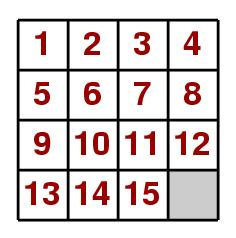
\includegraphics[width=4cm]{15grid}
	\centering
	\caption{Ułożona układanka. która jest też poprawnym rozwiązaniem.}
\end{figure}
\\
Przesuwanie elementów na planszy umożliwia puste pole. Układanie tych elementów można potraktować jak przeszukiwanie drzewa składającego się z węzłów o wartościach "R", "D", "U" oraz "L", które odpowiadają za przesunięcia pustego pola w prawo, dół, górę i lewo.

\section{Opis implementacji}
Program, który rozwiązuję układankę "Piętnastkę" został przez nas napisany w języku Python.\\
Zawiera on następujące klasy:
\begin{itemize}
	\item \textbf{Puzzle}
	\item \textbf{AStar}
\end{itemize}
\newpage
\subsection{Puzzle}
Klasa ta zawiera większość implementacji programu. Przede wszystkim, zawiera ona konstruktor układanki, który bierze pod uwagę takie parametry jak wymiary i wartości układanki, strategię oraz jej parametry, \\dodatkowe zmienne wykorzystywane w zapisie statystyk rozwiązania, oraz \\
Metody można podzielić na trzy zasadnicze funkcjonalności:
\begin{itemize}
	\item Operacje na plikach
	\item Poruszanie się po planszy
	\item Algorytmy rozwiązania układanki
\end{itemize}
W tej klasie są cztery najważniejsze metody: \texttt{bfs}, \texttt{dfs}, \texttt{aStar} oraz \texttt{moveNode}.
Metoda \texttt{bfs} implementuje algorytm BFS do rozwiązania układanki. Podobną implementację ma metoda \texttt{dfs}, która odpowiada za algorytm DFS. \\
\texttt{aStar} jest odpowiedzialna za utworzenie obiektu klasy AStar, który wywołuję metodę \texttt{solve} do rozwiązania układu. Metoda \texttt{moveNode} pozwala na poruszanie pustym polem po planszy, po czym zwraca plansze z wykonanym ruchem.

\subsection{AStar}
Klasa ta implementuje trzy najważniejsze metody: \texttt{manhattanDistance}, \texttt{hammingDistance} oraz \texttt{solve}. \texttt{manhattanDistance} oraz \texttt{hammingDistance} odpowiadają za implementację heurystyk Hamminga oraz Manhattan wymagane do algorytmu A*. Metoda \texttt{solve} implementuje algorytm A*, który korzysta właśnie z tych heurystyk.

\section{Materiały i metody}
Badania zostały przeprowadzone przy użyciu załączonych skryptów \texttt{bash}, które były do pobrania na stronie przedmiotu. Wygenerowaliśmy wszystkie możliwe układanki dla ruchów od 1 do 7, czyli łącznie 413 układanek.\\
Następnie przy pomocny skryptu "Uruchamiacz przeszukiwań" uruchomiliśmy naszą aplikacji dla następujących parametrów:\\
\begin{itemize}
	\item \textbf{Algorytmy BFS i DFS}
	\begin{itemize}
		\item \textit{prawo-dół-góra-lewo;}
		\item \textit{prawo-dół-lewo-góra;}
		\item \textit{dół-prawo-góra-lewo;}
		\item \textit{dół-prawo-lewo-góra.}
		\item \textit{lewo-góra-dół-prawo.}
		\item \textit{lewo-góra-prawo-dół;}
		\item \textit{góra-lewo-dół-prawo;}
		\item \textit{góra-lewo-prawo-dół;}
	\end{itemize}
	\item \textbf{Algorytm A*}
	\begin{itemize}
		\item{Metryka Hamminga}
		\item{Metryka Manhattan}
	\end{itemize}
\end{itemize}
\newpage

\setcounter{figure}{0}

\section{Wyniki}
Wyniki naszych badań zostały przedstawione na wykresach poniżej. \\
Podzieliliśmy je ze względu na wykorzystaną strategię przeszukiwania.\\ 
Na każdym wykresie oś X przedstawia odległość początkowej układanki \\
od rozwiązania.
\begin{figure}[ht]
	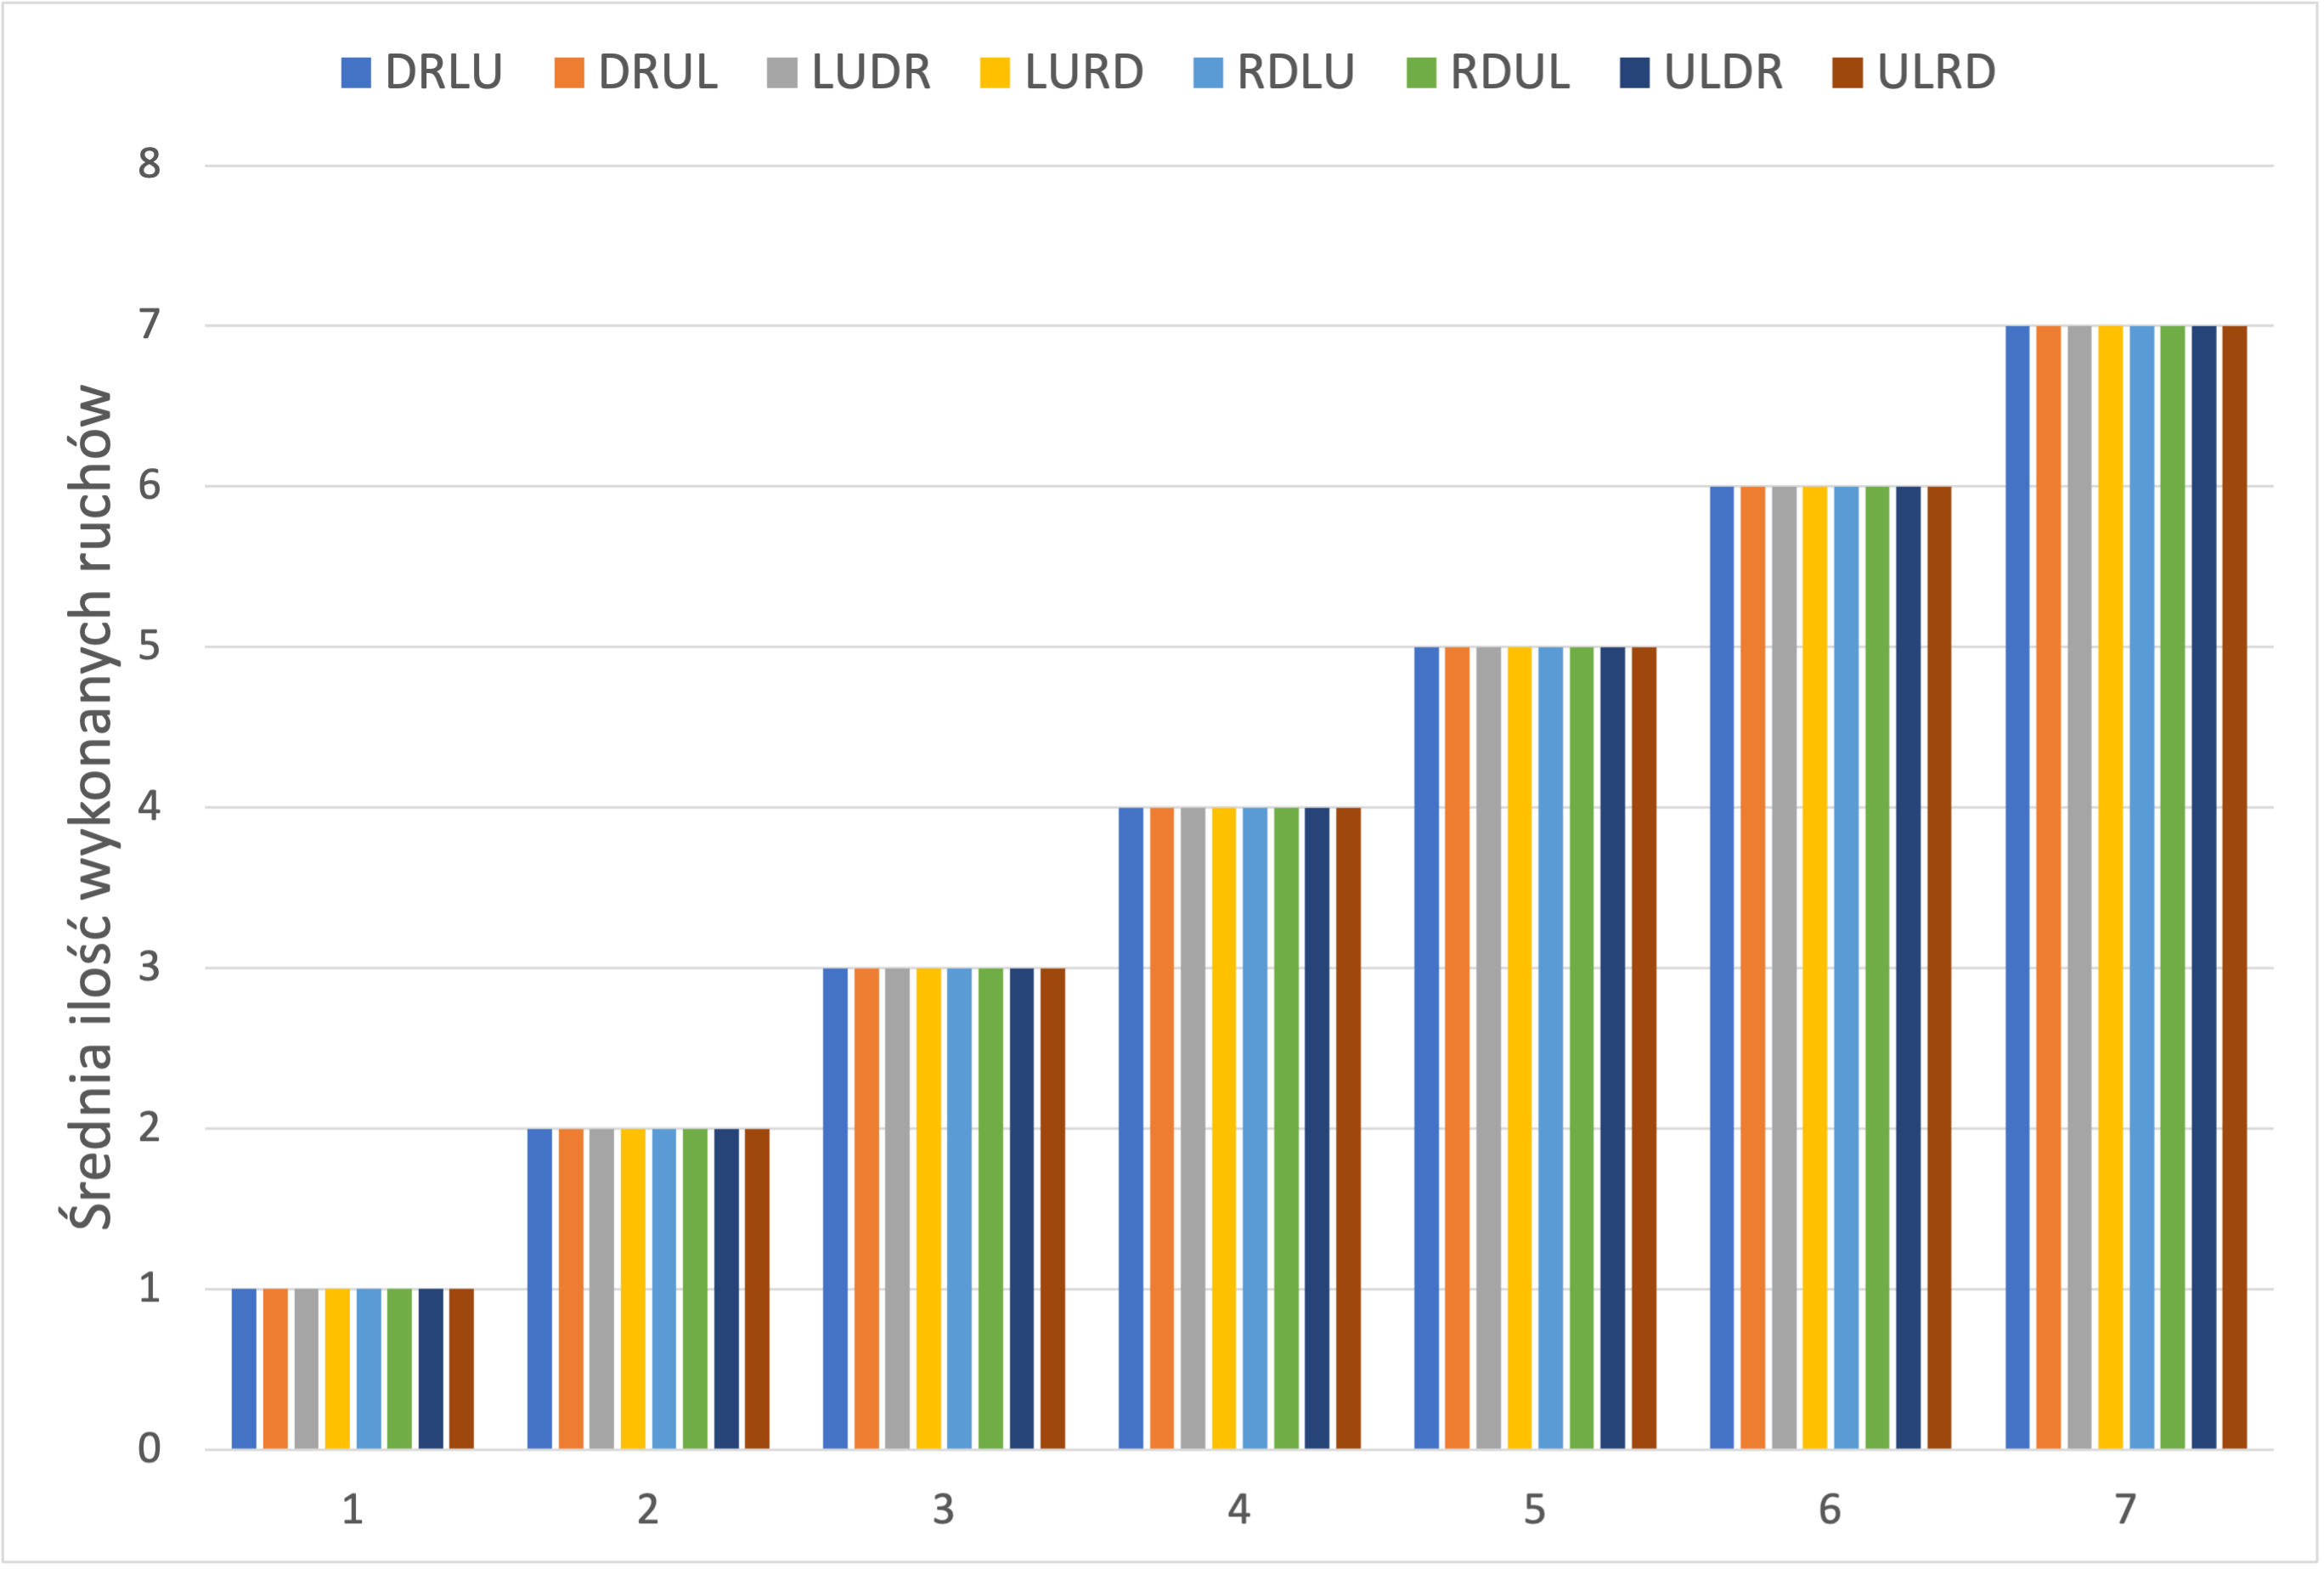
\includegraphics[width=11cm]{BFS/BFS_śr_ruchów}
	\centering
	\captionsetup{name=Wykres}
	\caption{Średnia liczba wykonanych ruchów dla BFS.}
		
	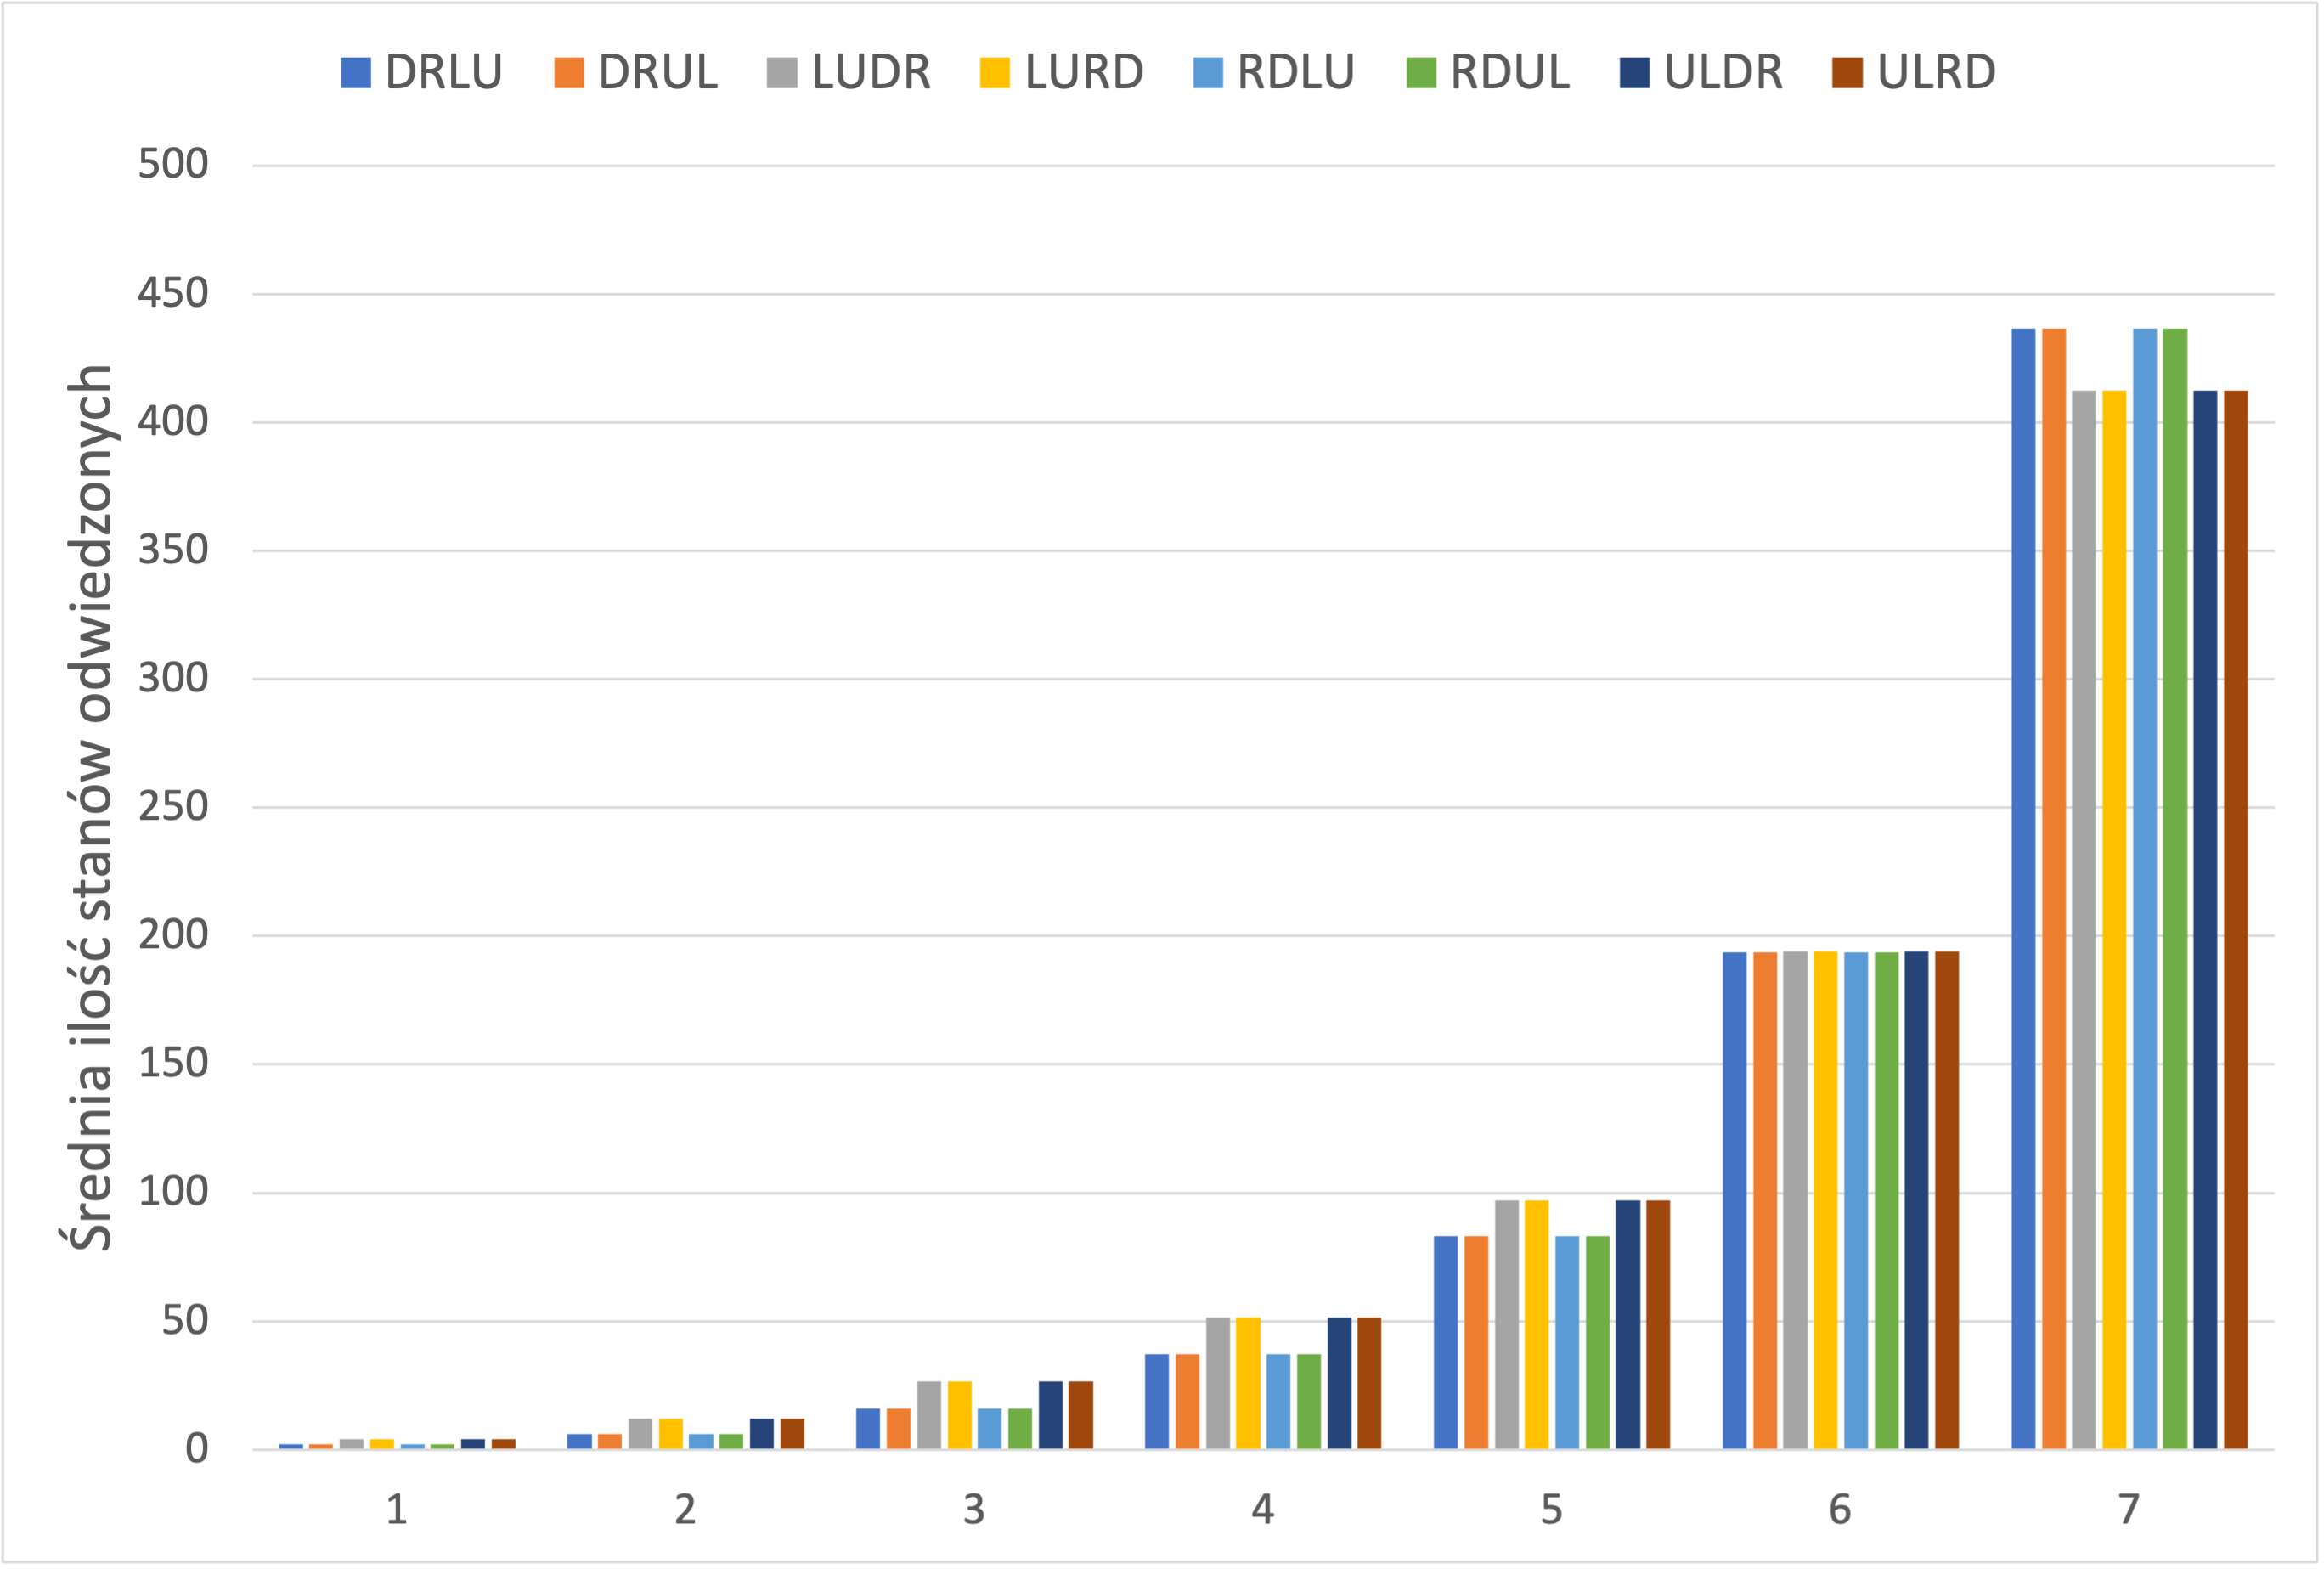
\includegraphics[width=11cm]{BFS/BFS_odwiedzone}
	\centering
	\captionsetup{name=Wykres}
	\caption{Średnia liczba odwiedzonych stanów dla BFS.}
\end{figure}
\begin{figure}
	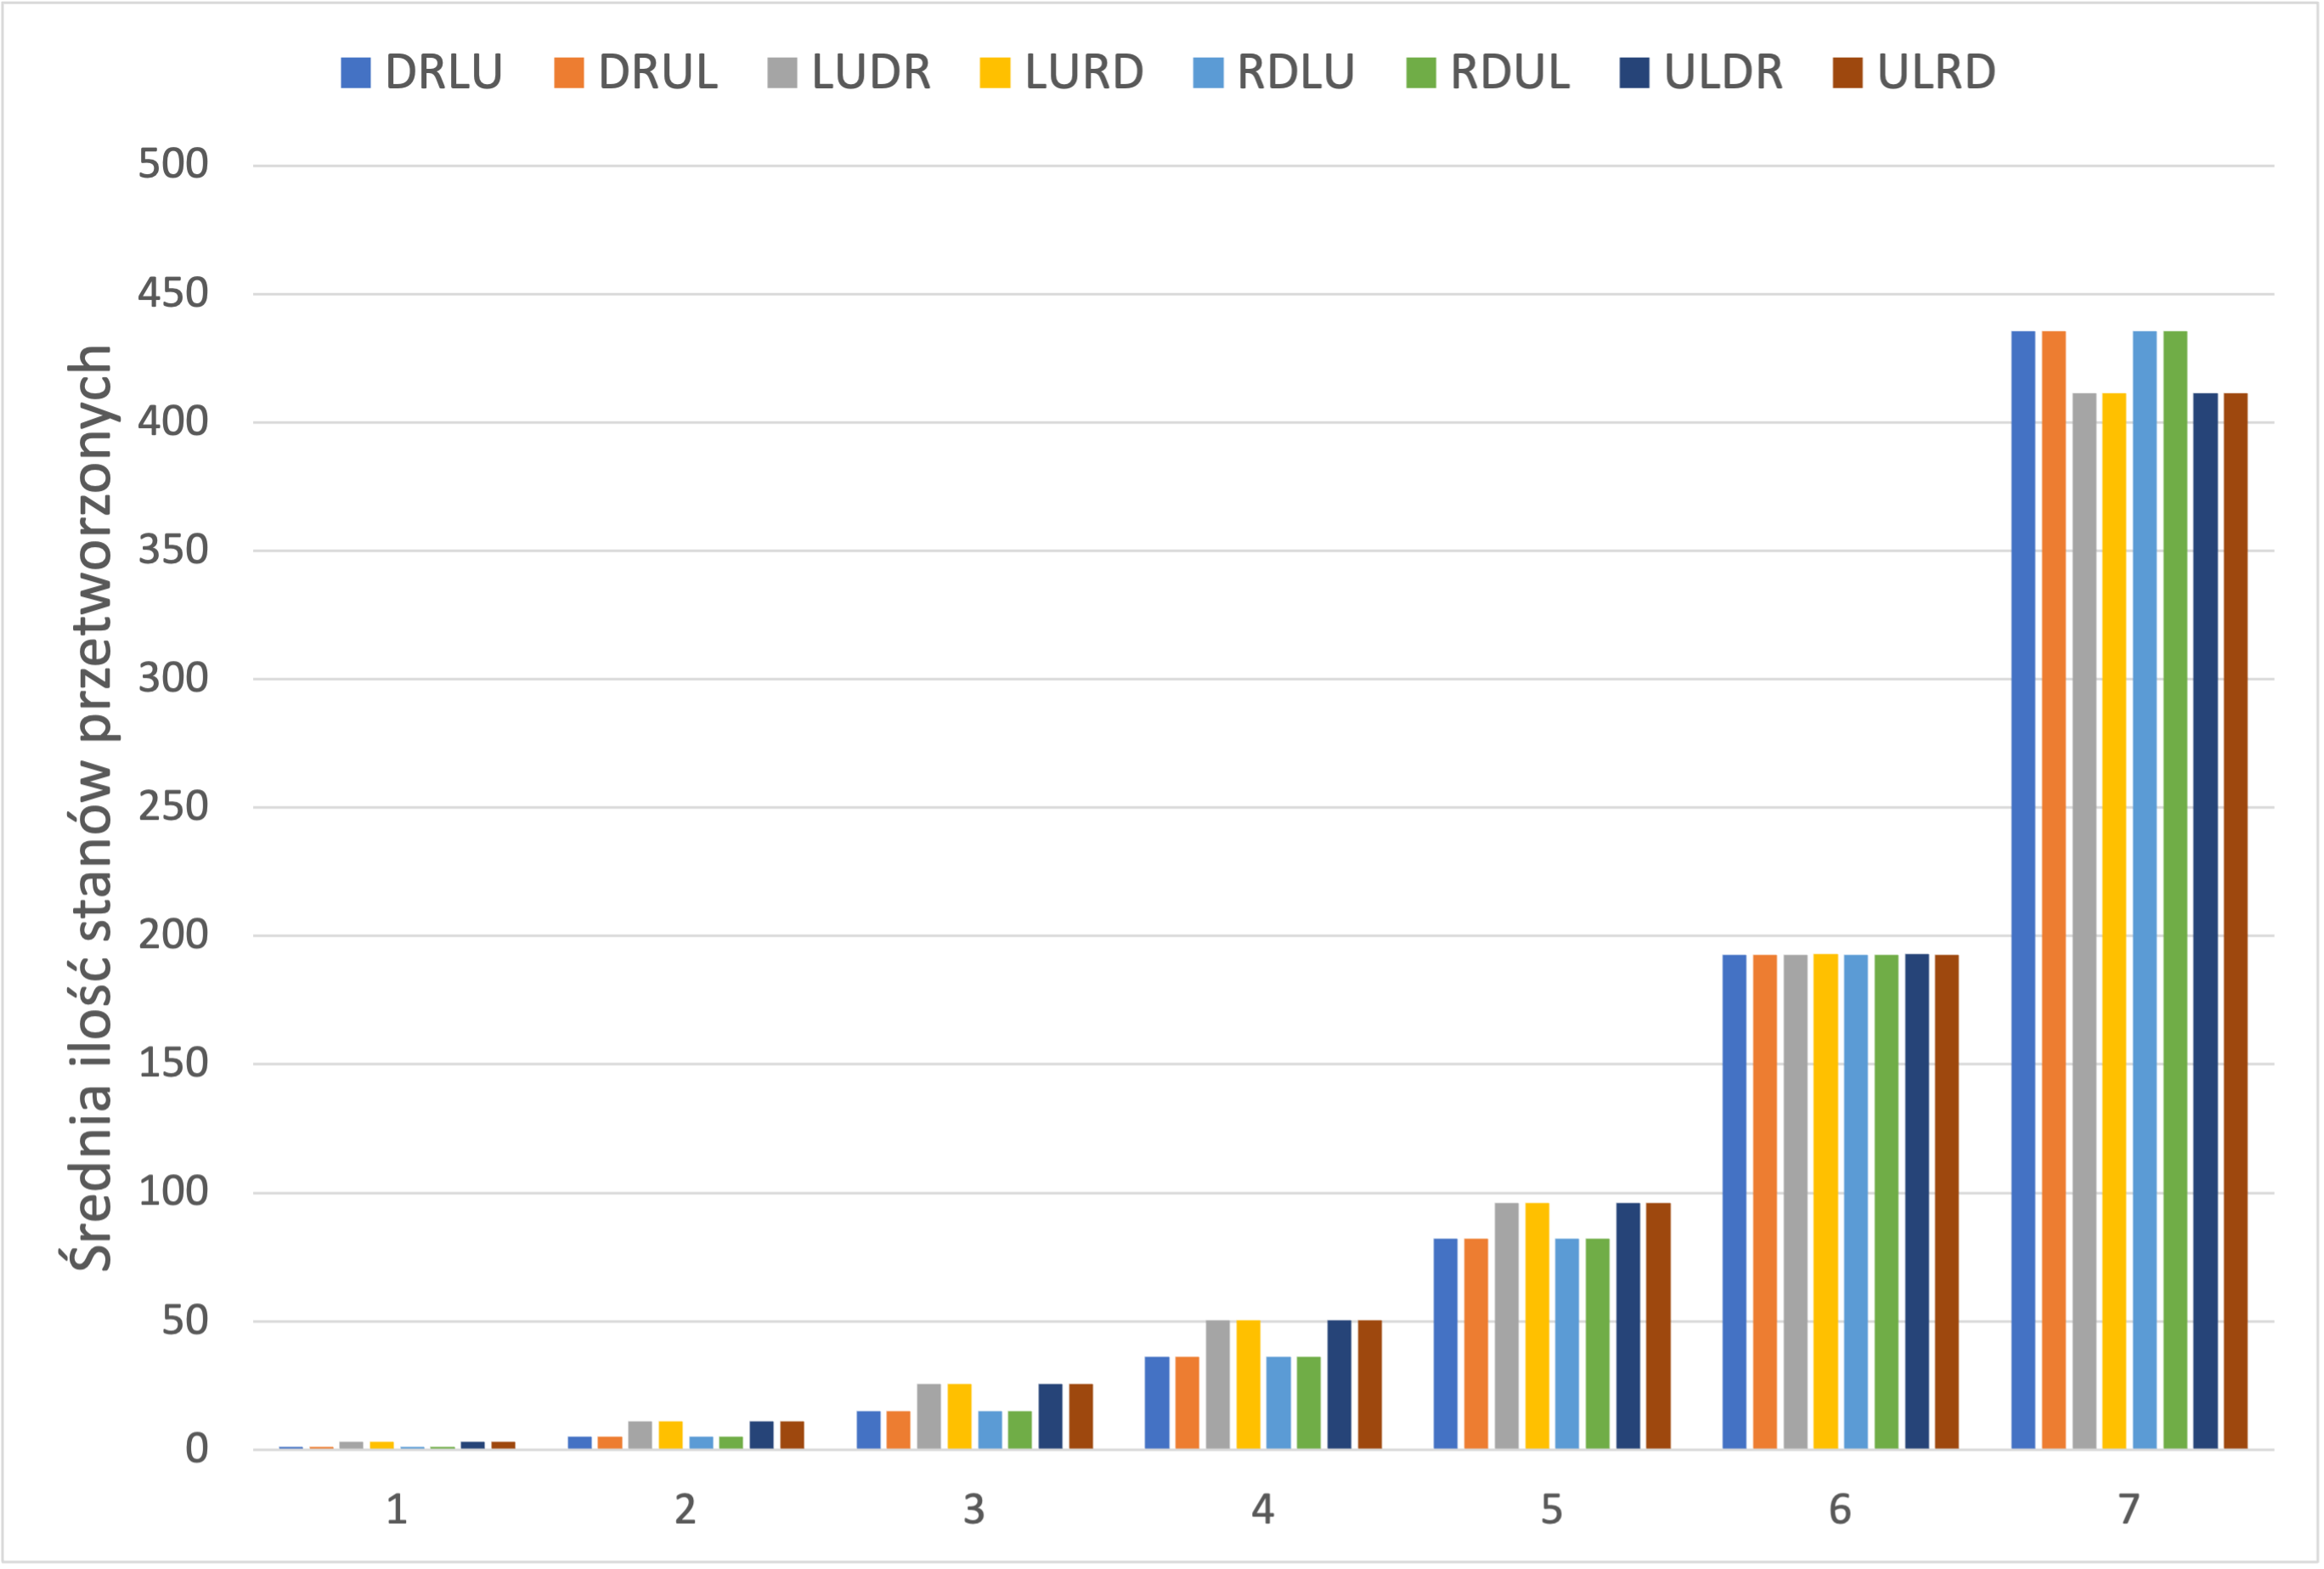
\includegraphics[width=11cm]{BFS/BFS_przetworzone}
	\centering
	\captionsetup{name=Wykres}
	\caption{Średnia liczba przetworzonych stanów dla BFS.}
		
	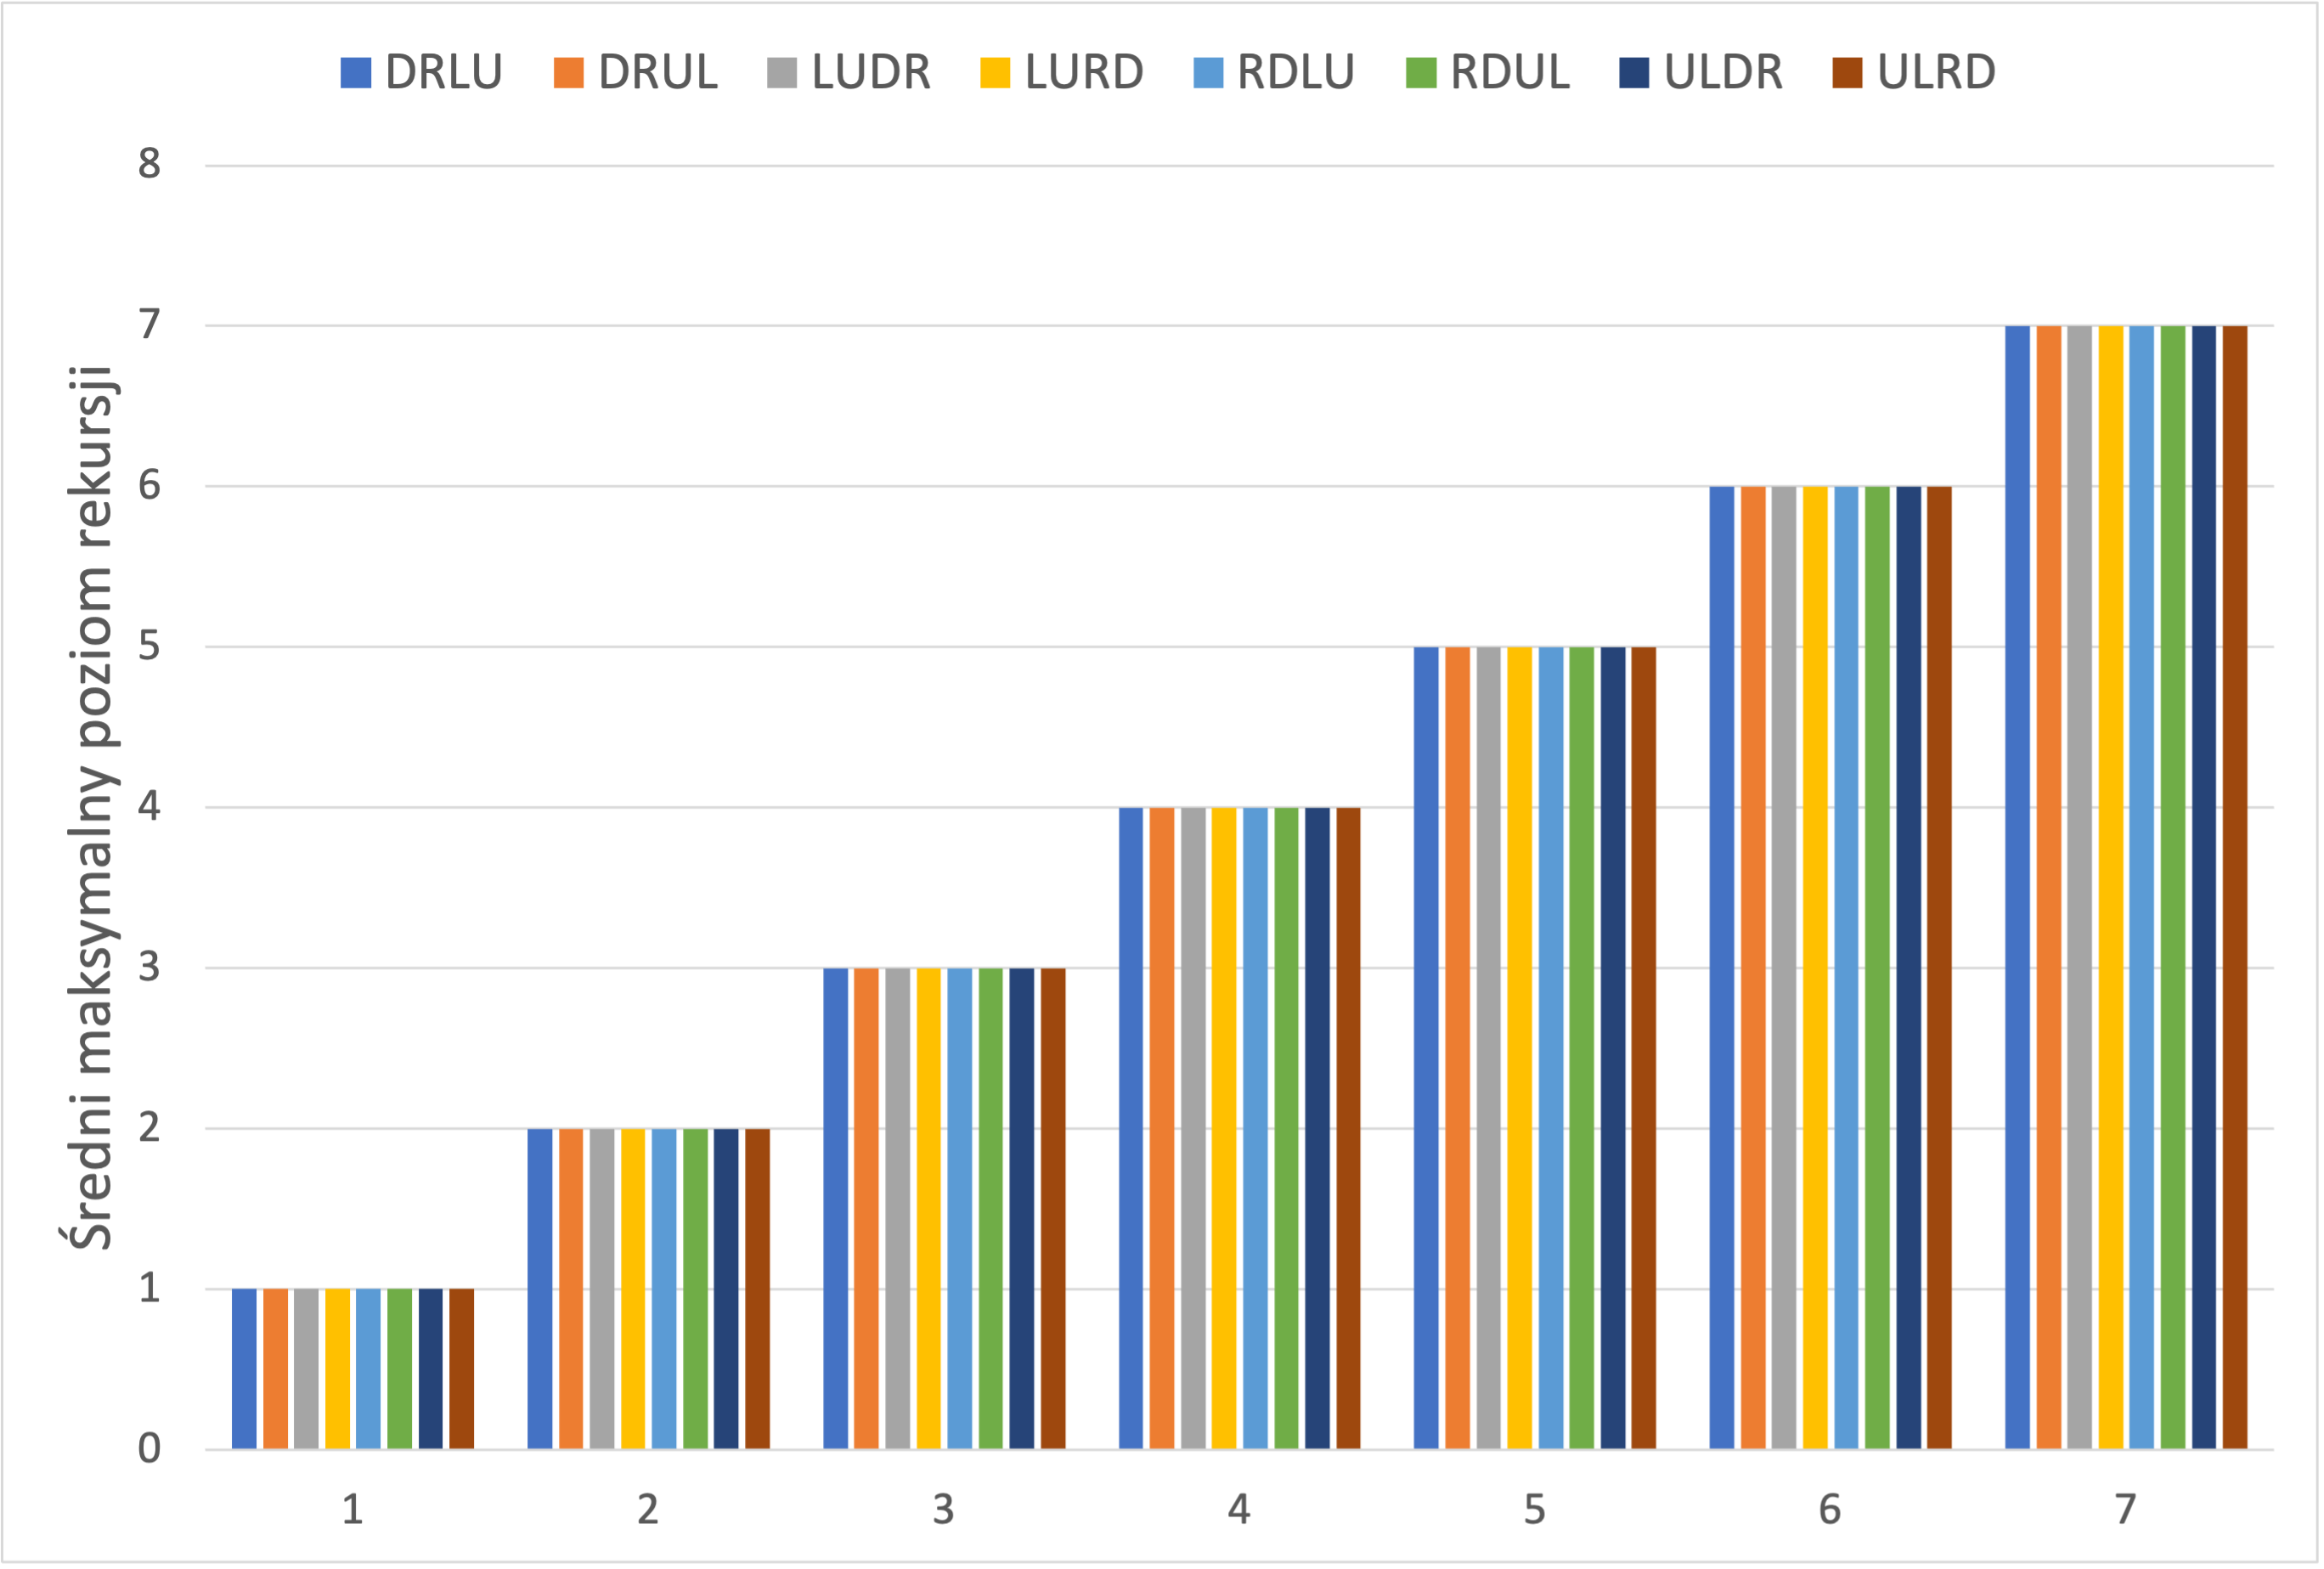
\includegraphics[width=11cm]{BFS/BFS_poziom_rekursji}
	\centering
	\captionsetup{name=Wykres}
	\caption{Średni maksymalny poziom rekursji dla BFS.}
		
	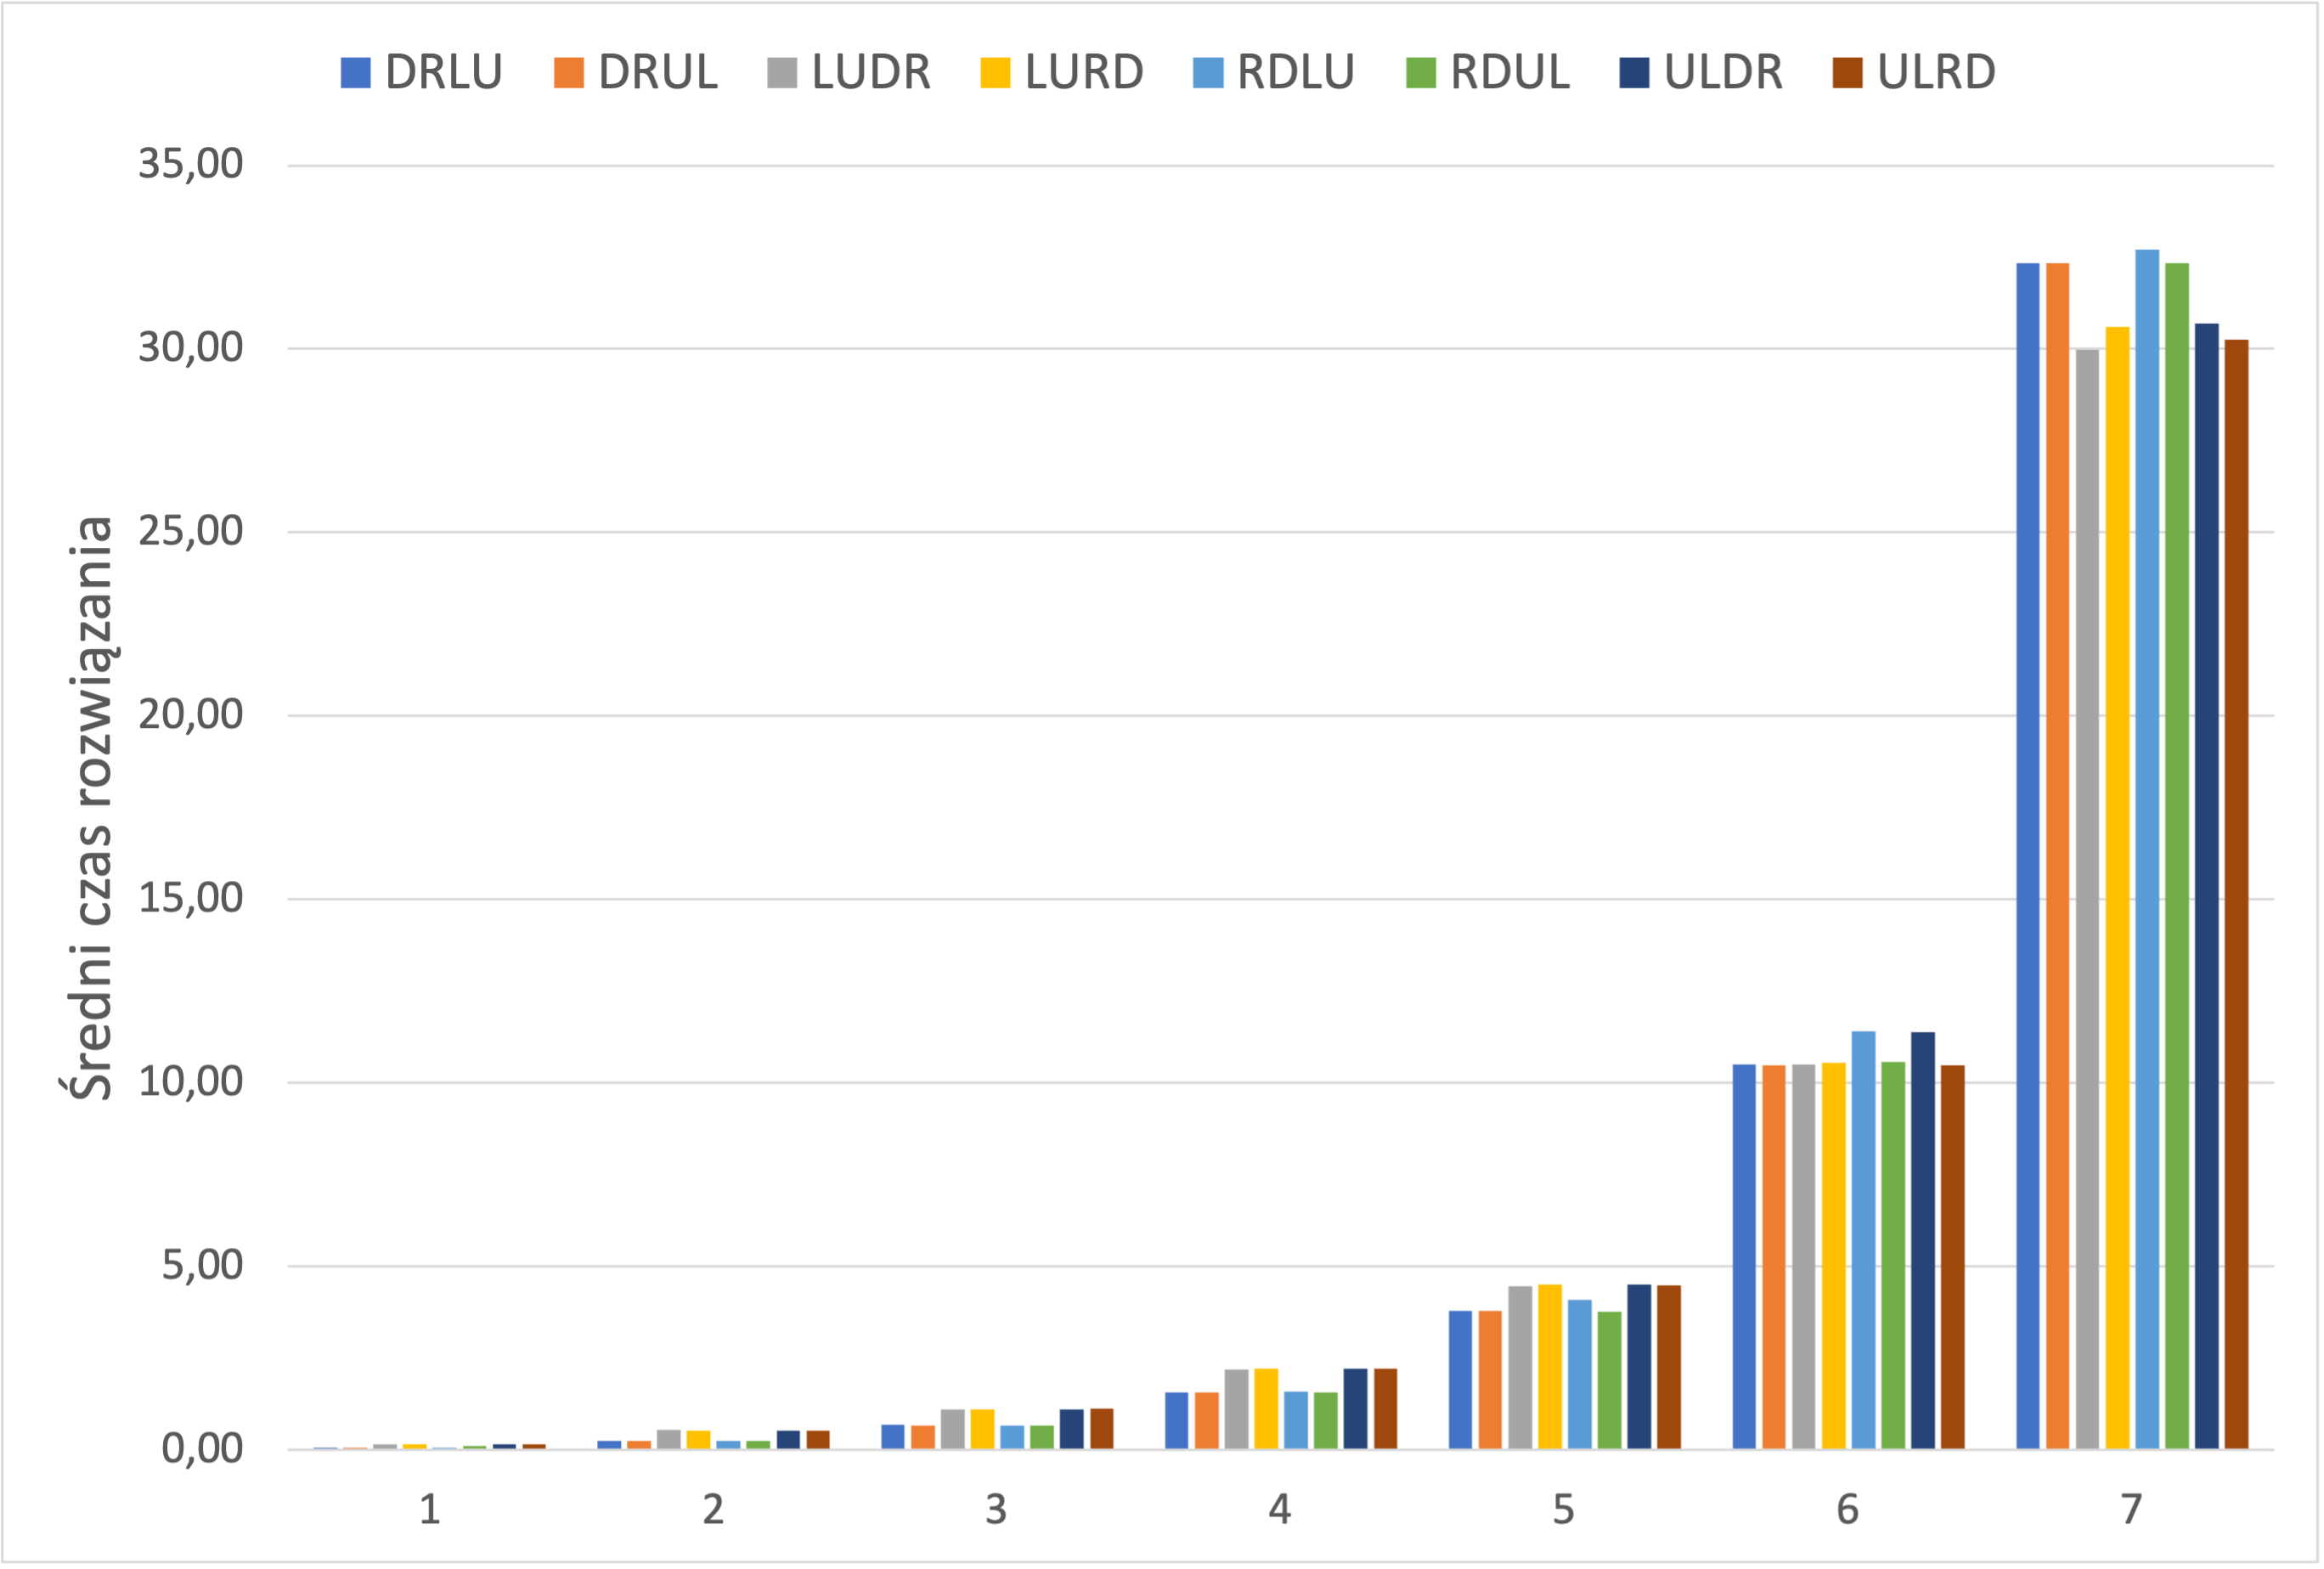
\includegraphics[width=11cm]{BFS/BFS_czas}
	\centering
	\captionsetup{name=Wykres}
	\caption{Średni czas rozwiązania dla BFS.}
\end{figure}
\begin{figure}
	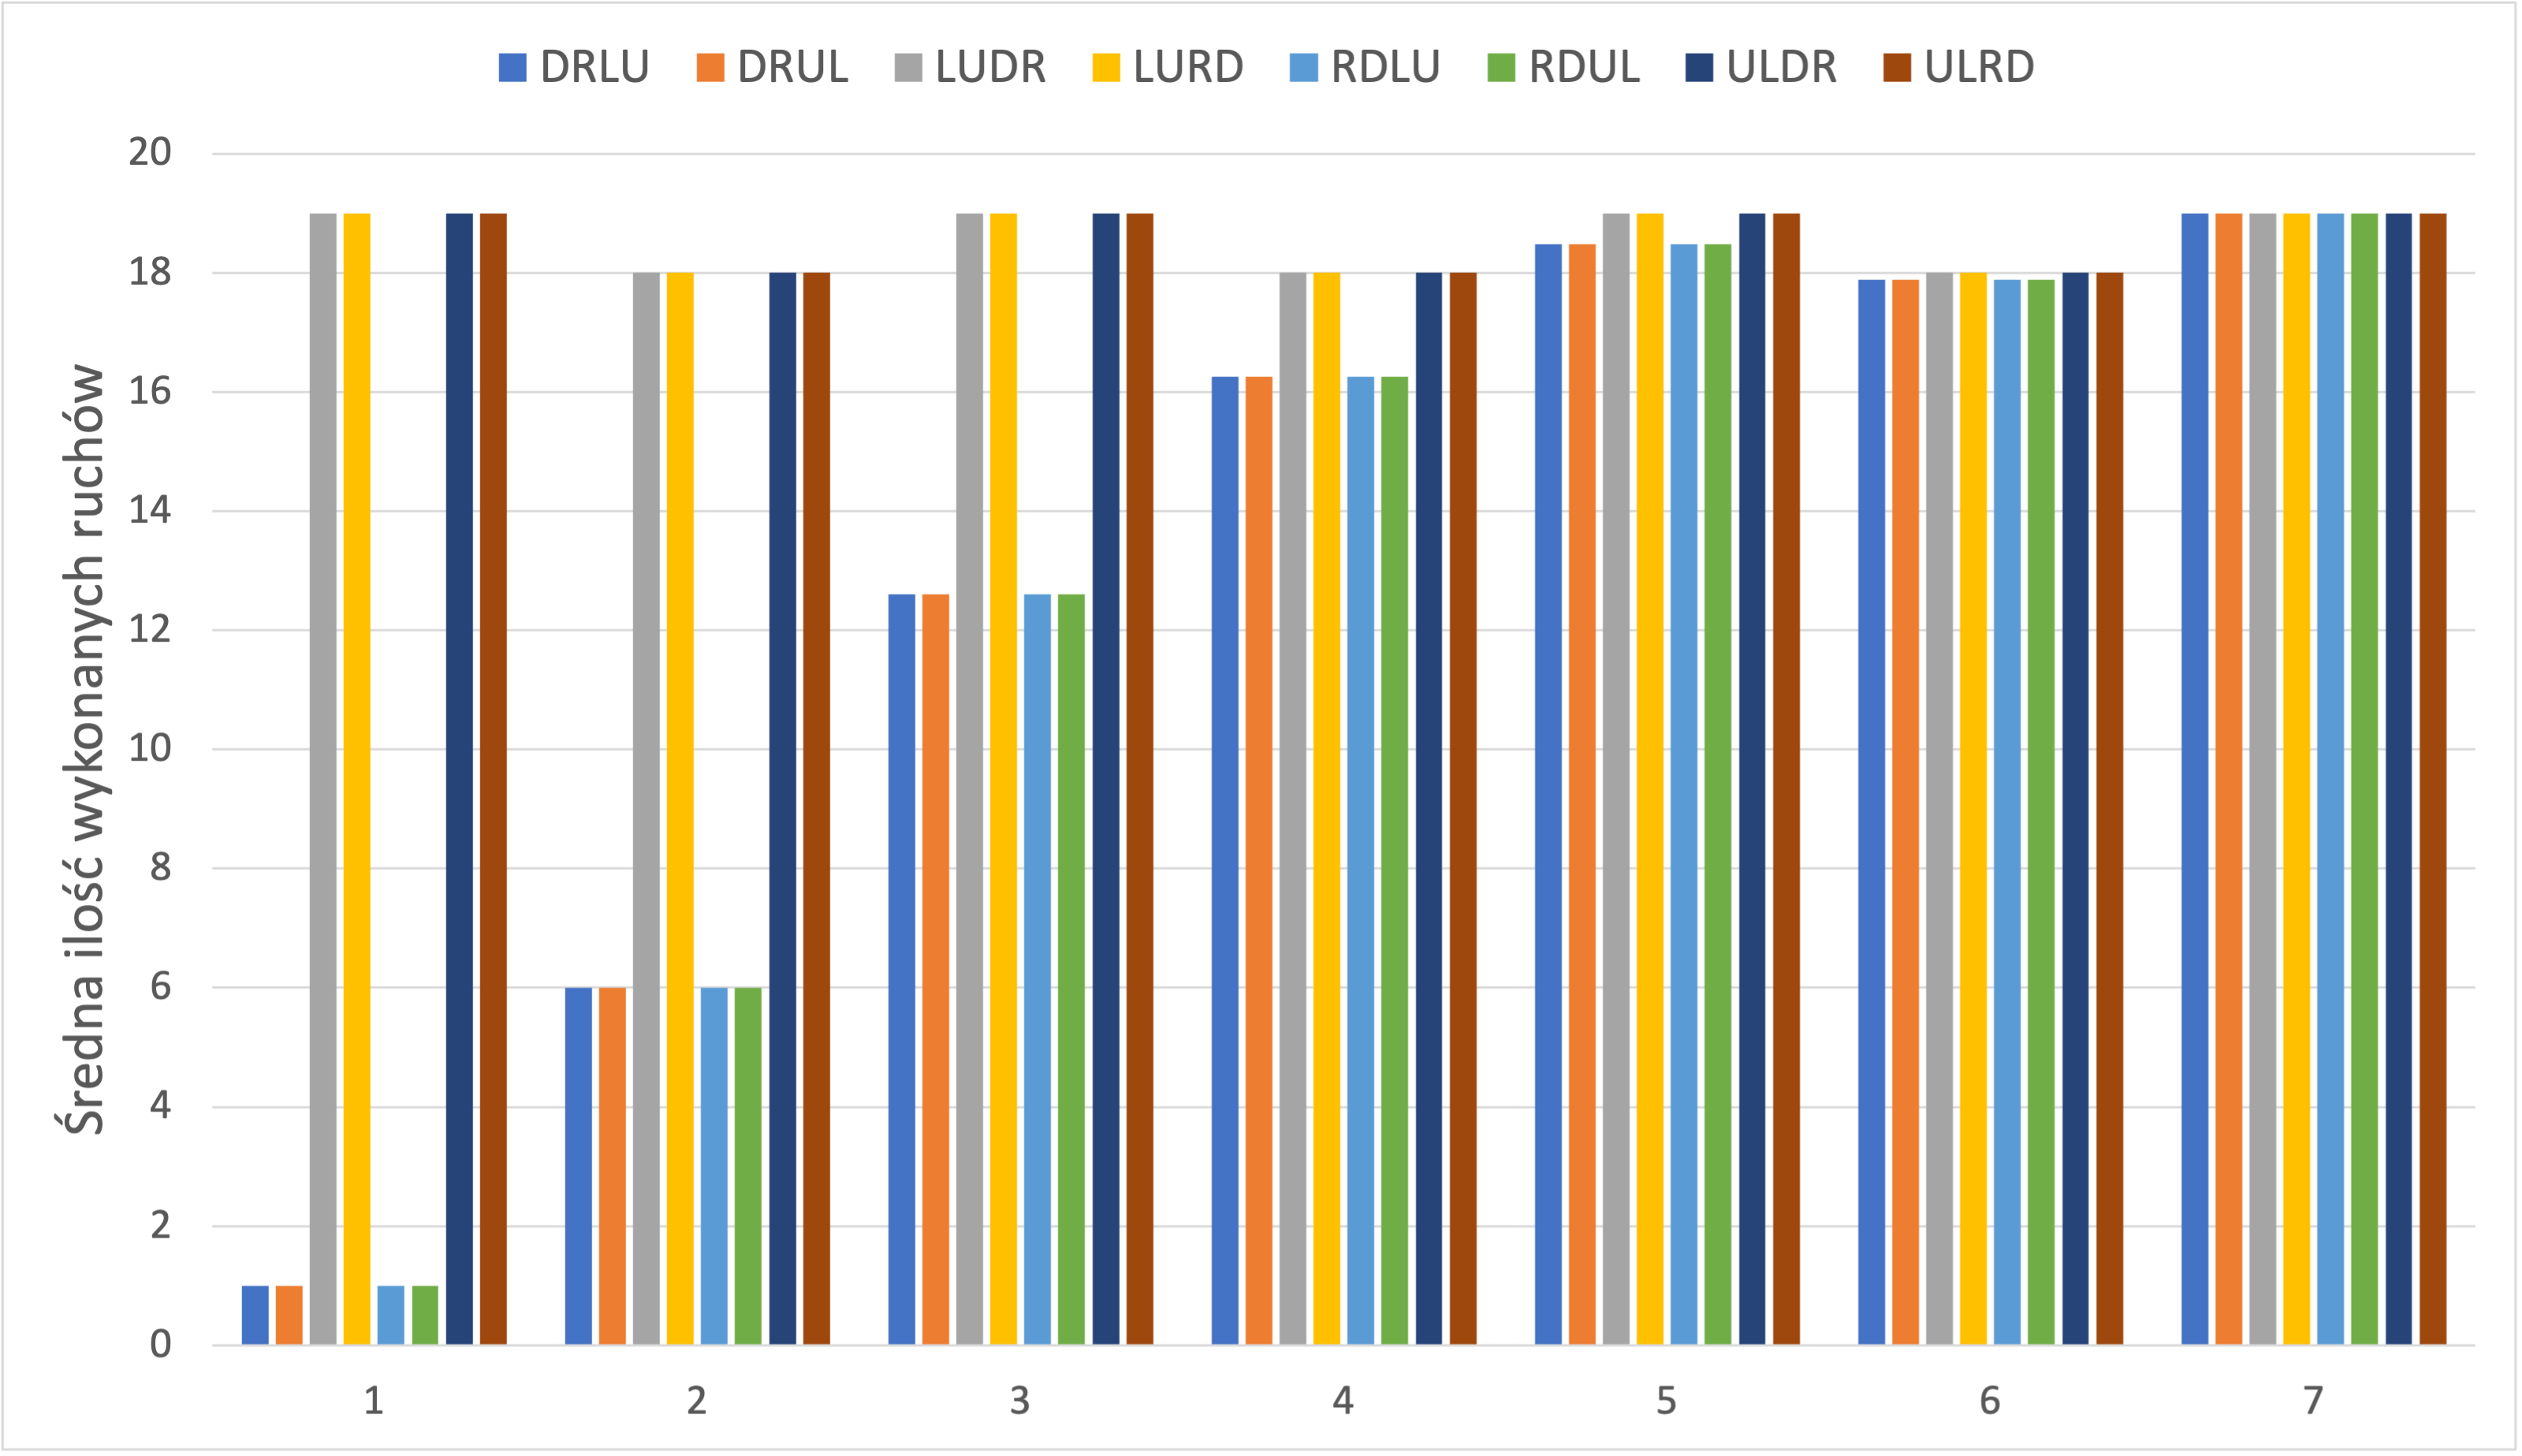
\includegraphics[width=11cm]{DFS/DFS_śr_ruchów}
	\centering
	\captionsetup{name=Wykres}
	\caption{Średnia liczba wykonanych ruchów dla DFS.}
		
	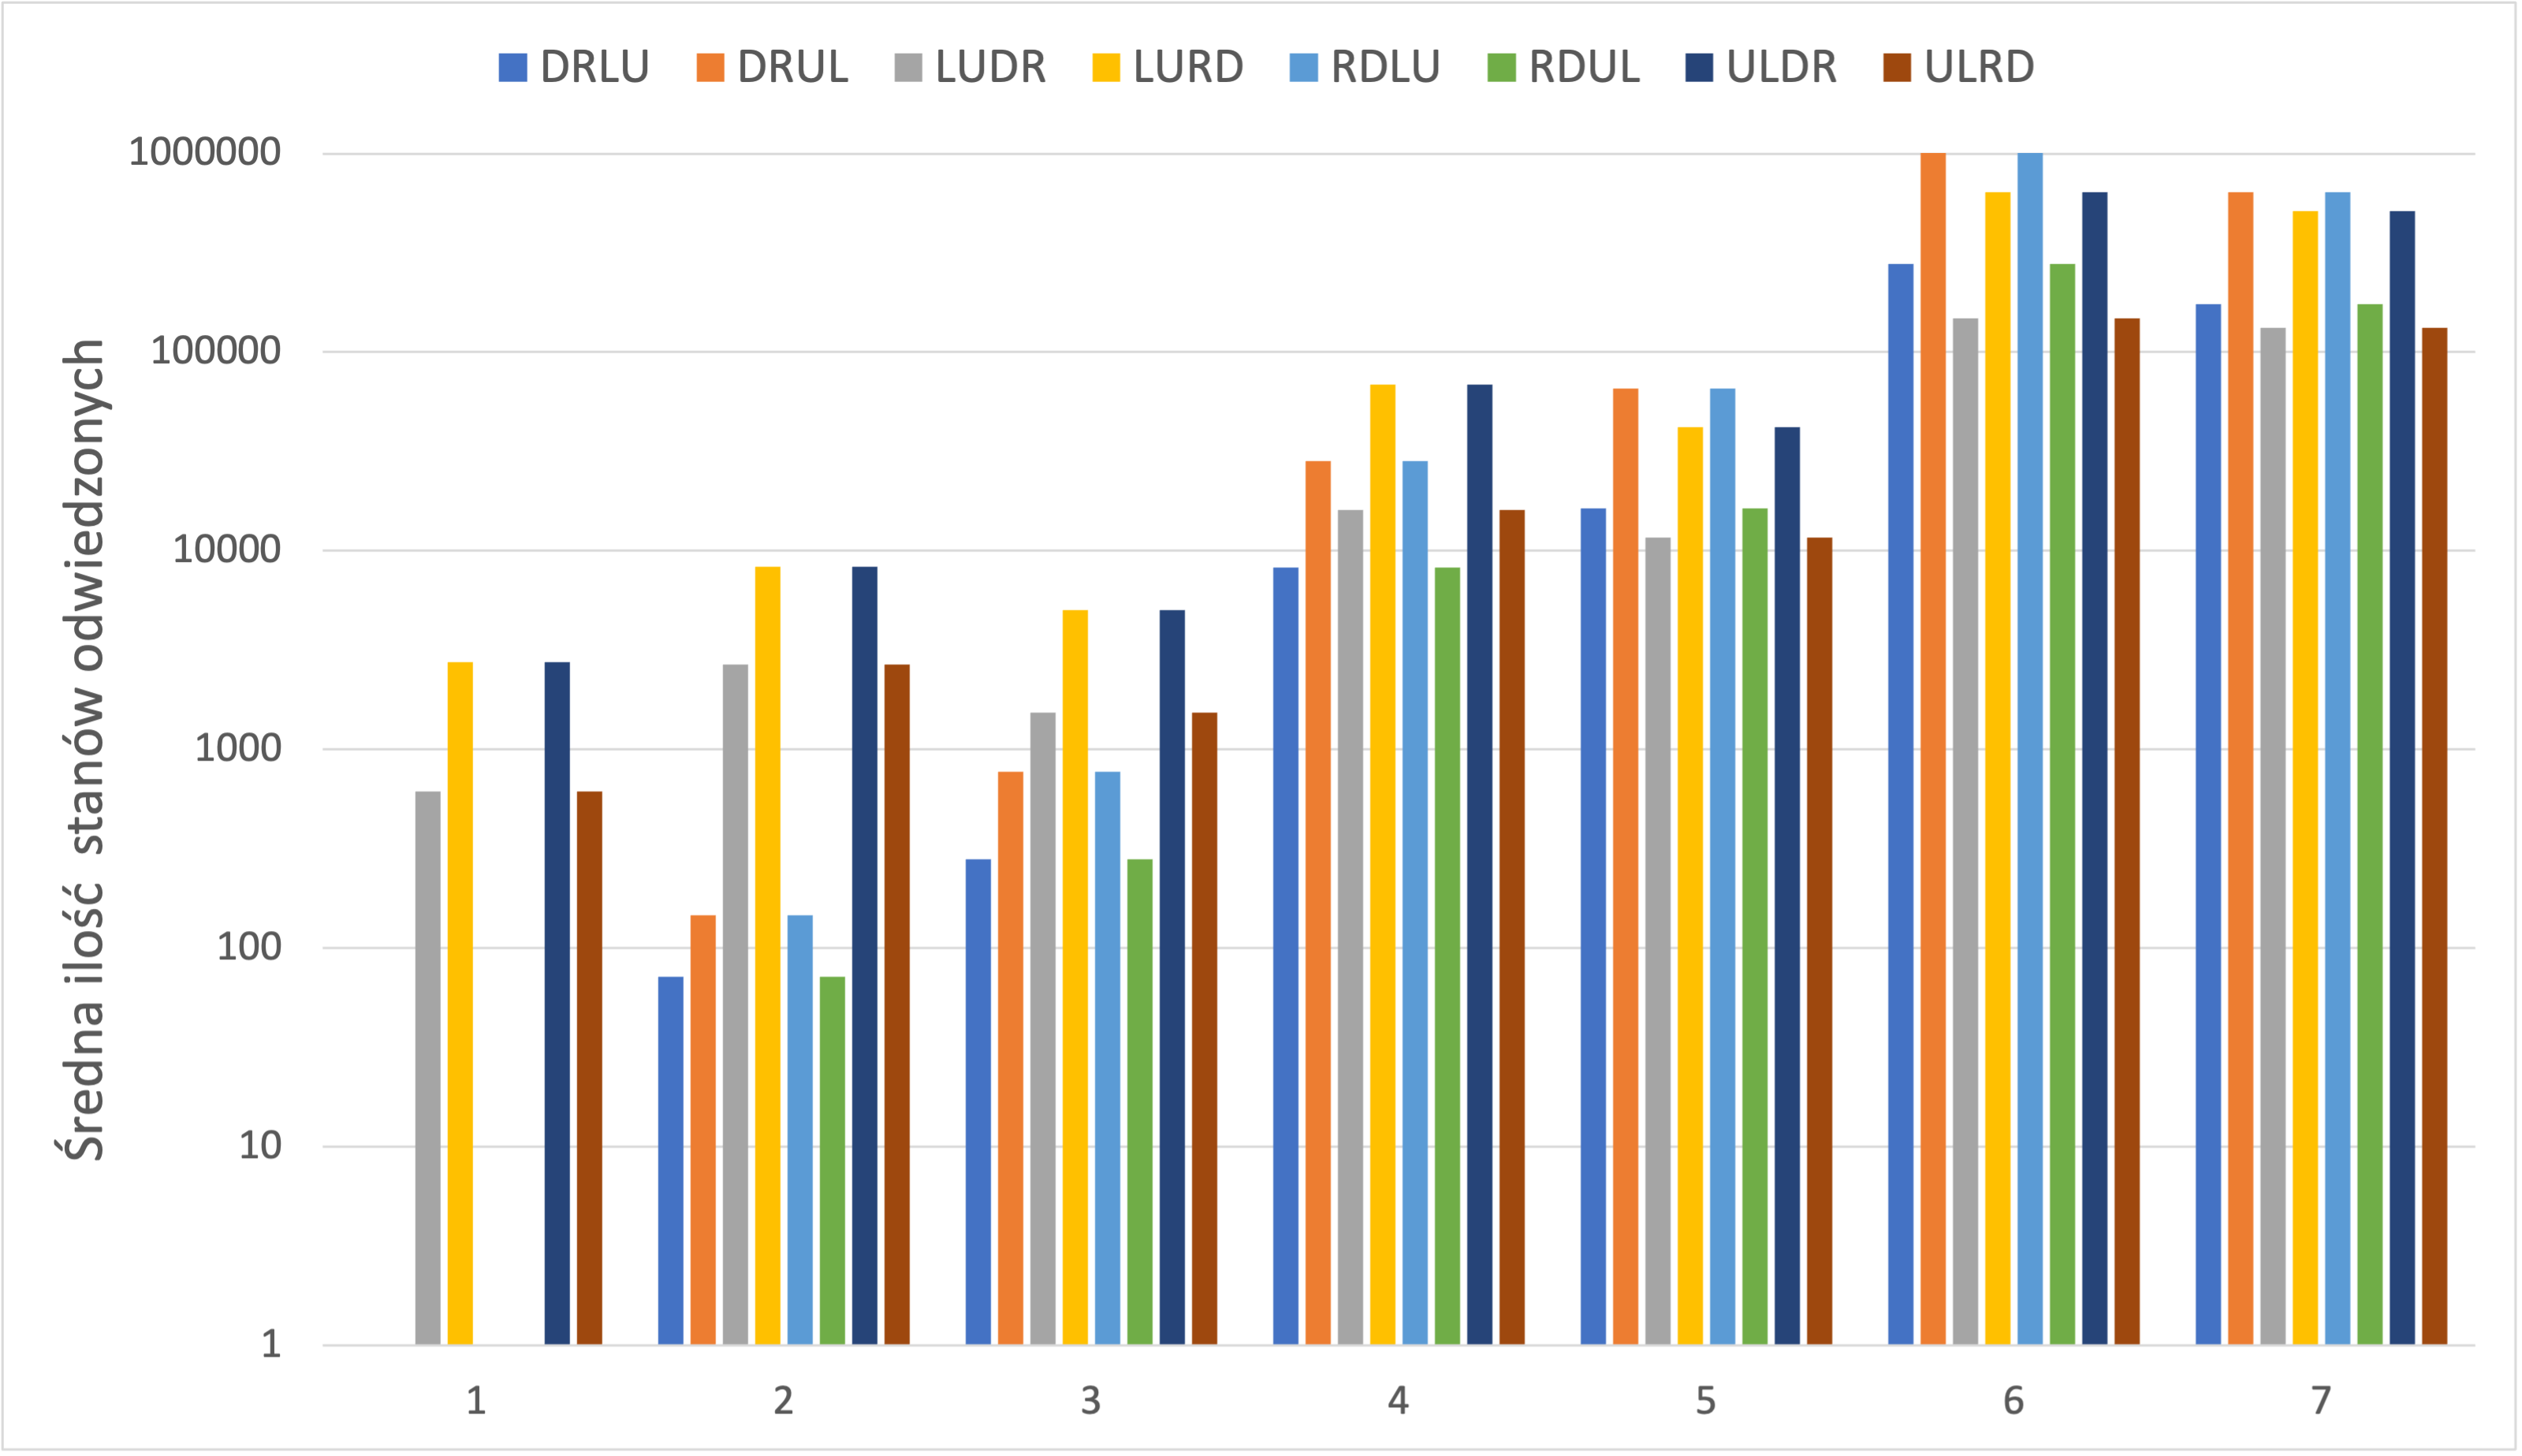
\includegraphics[width=11cm]{DFS/DFS_odwiedzone}
	\centering
	\captionsetup{name=Wykres}
	\caption{Średnia liczba odwiedzonych stanów dla DFS.}
	
	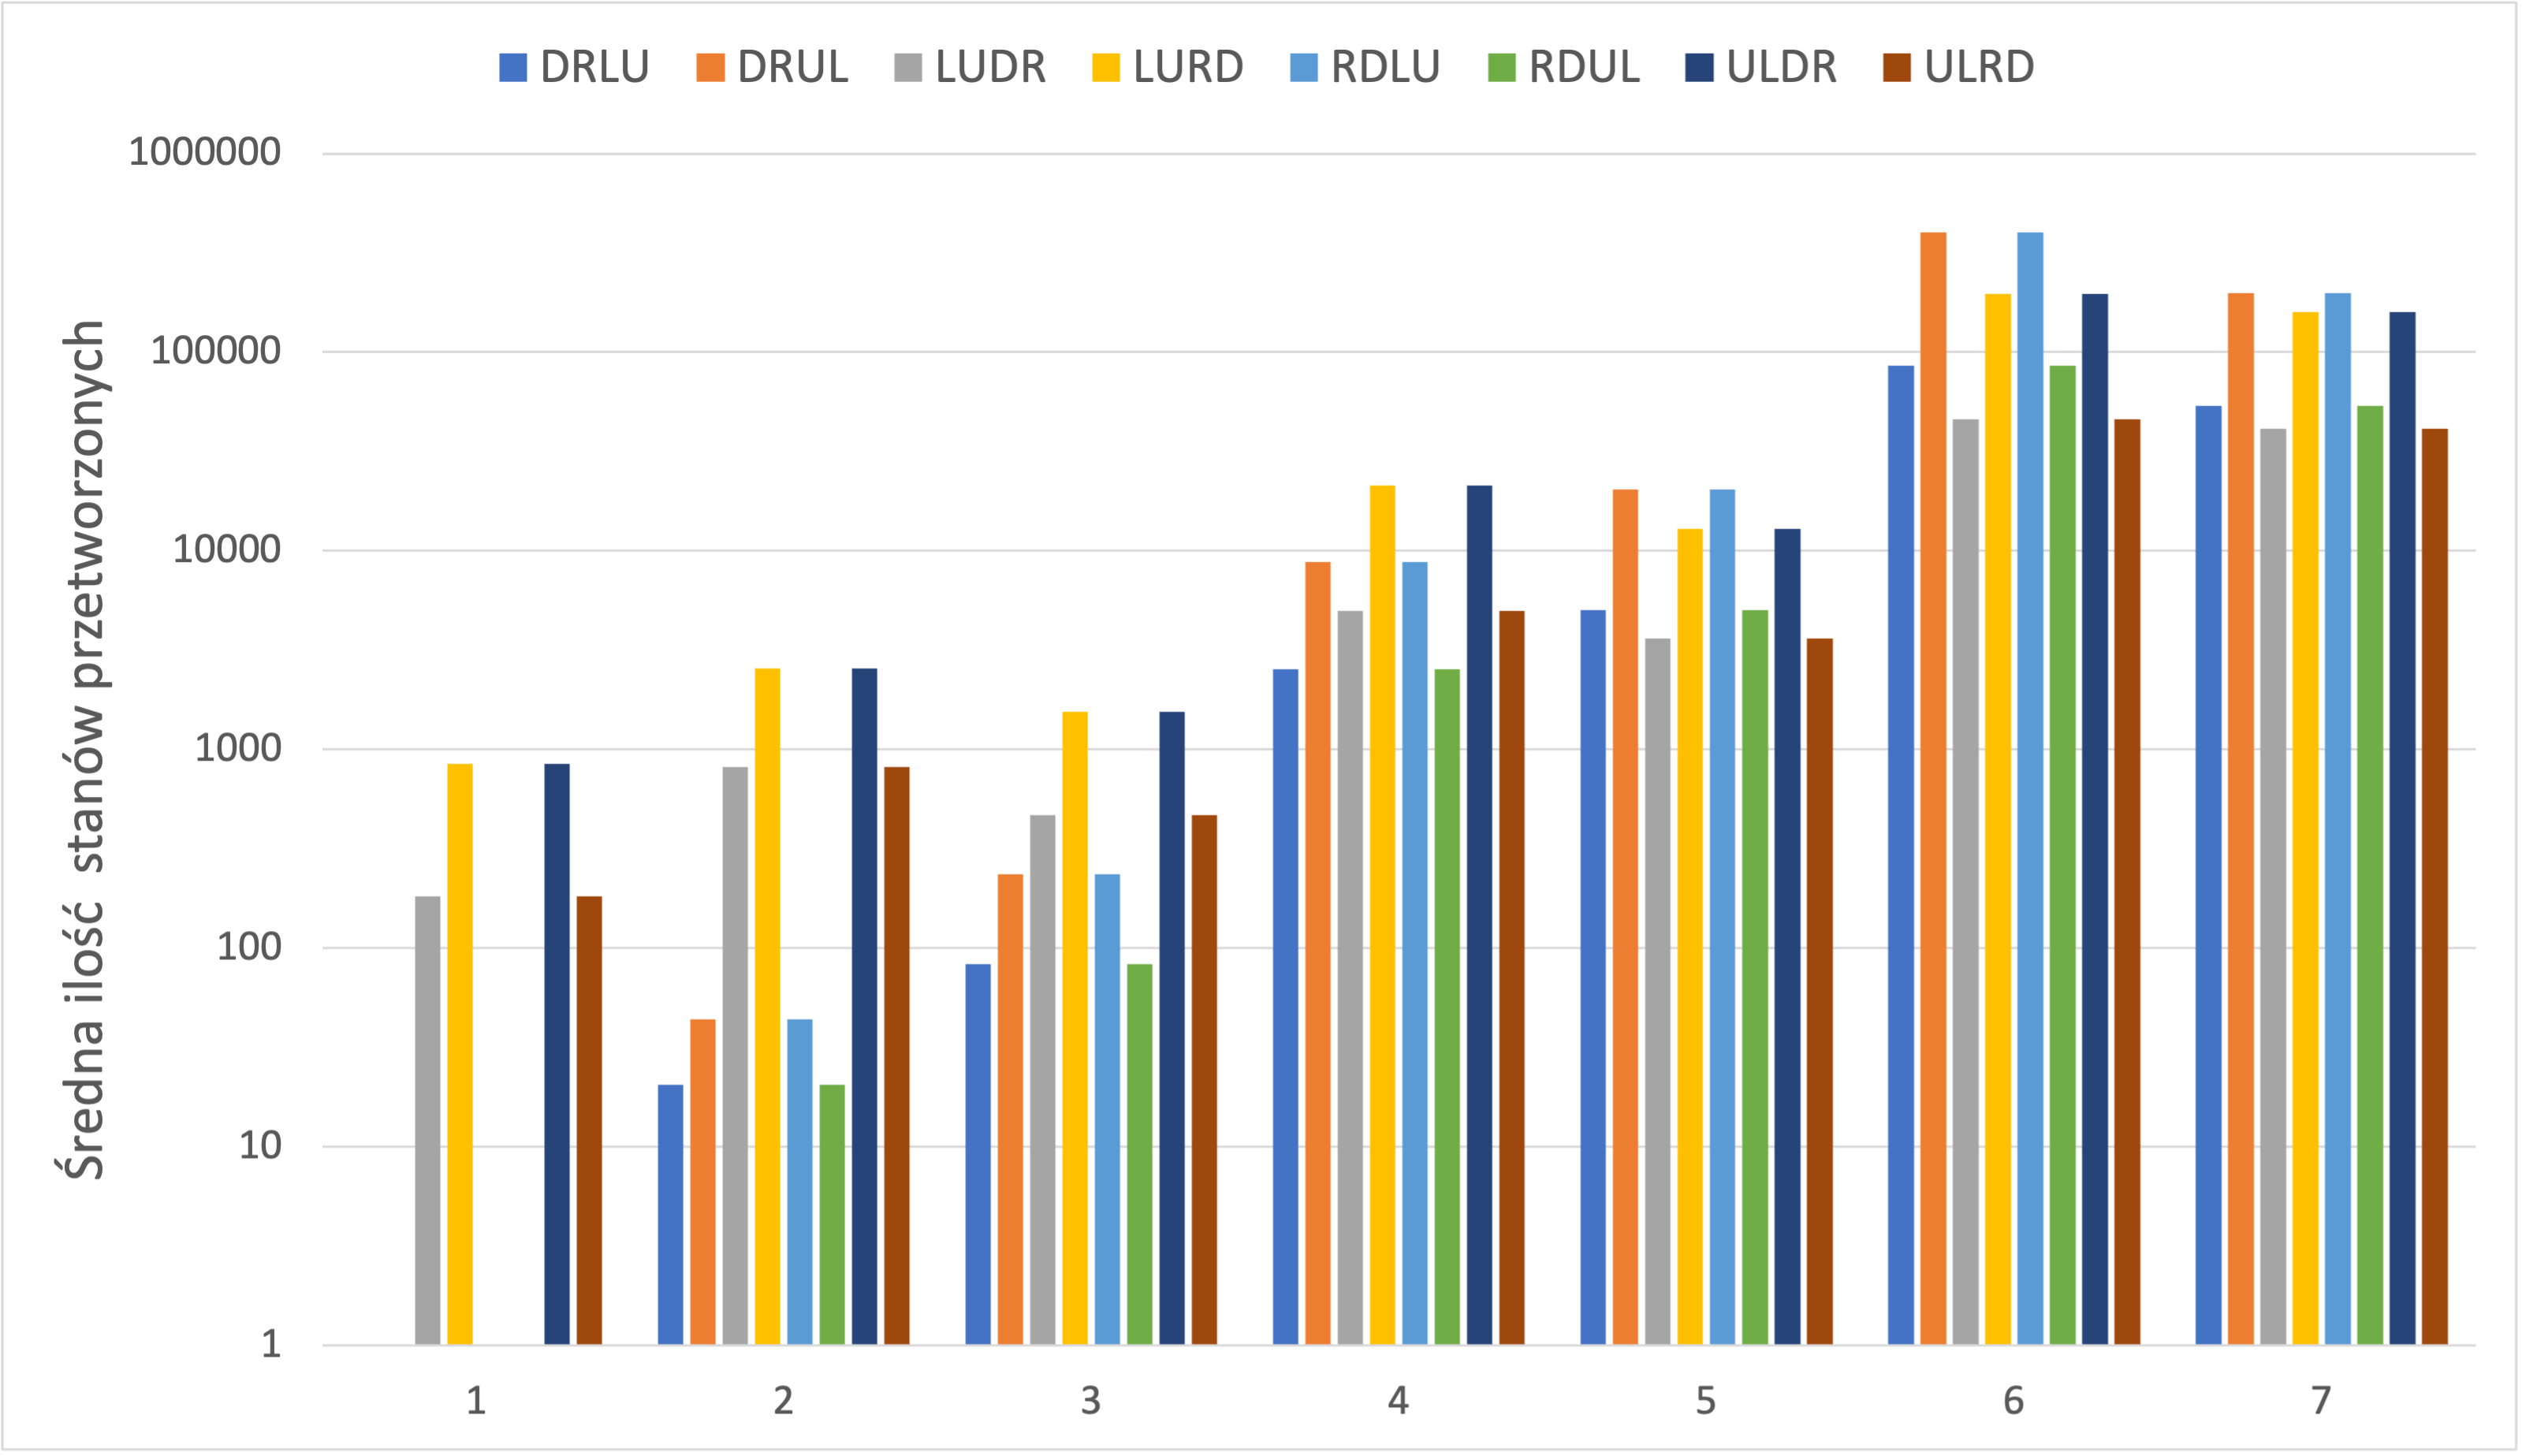
\includegraphics[width=11cm]{DFS/DFS_przetworzone}
	\centering
	\captionsetup{name=Wykres}
	\caption{Średnia liczba przetworzonych stanów dla DFS.}
\end{figure}
\begin{figure}
	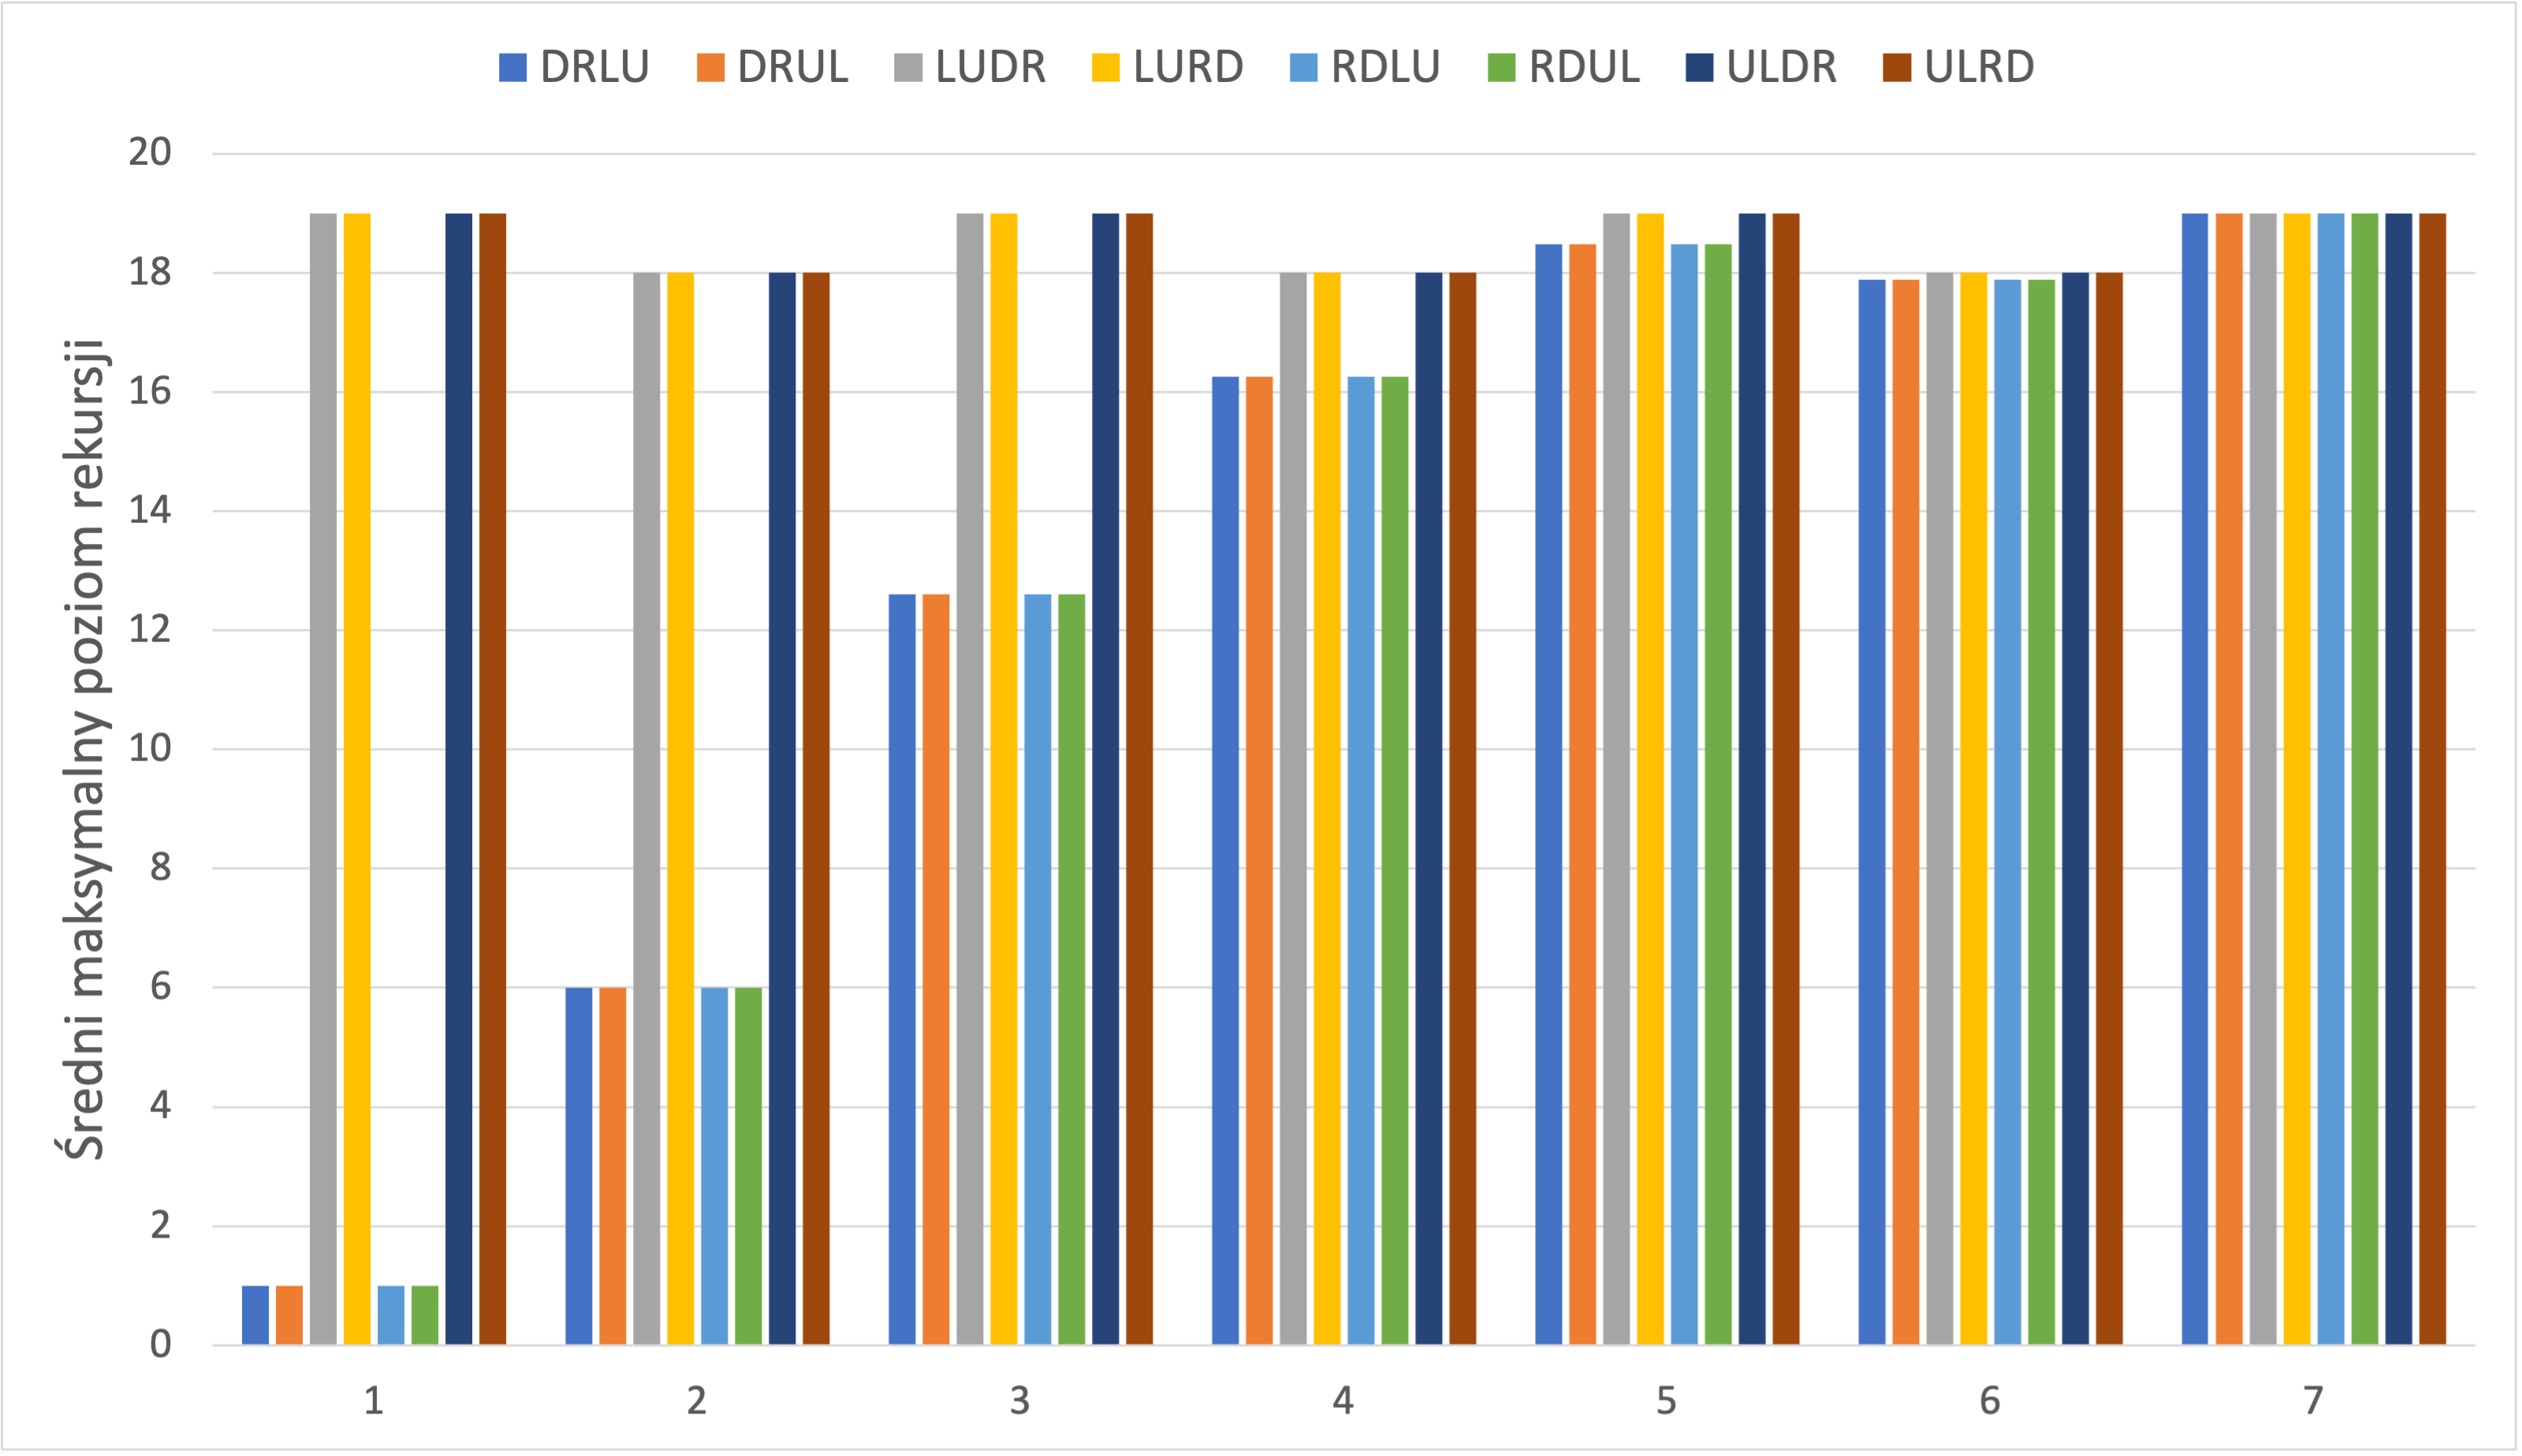
\includegraphics[width=11cm]{DFS/DFS_poziom_rekursji}
	\centering
	\captionsetup{name=Wykres}
	\caption{Średni maksymalny poziom rekursji dla DFS.}
		
	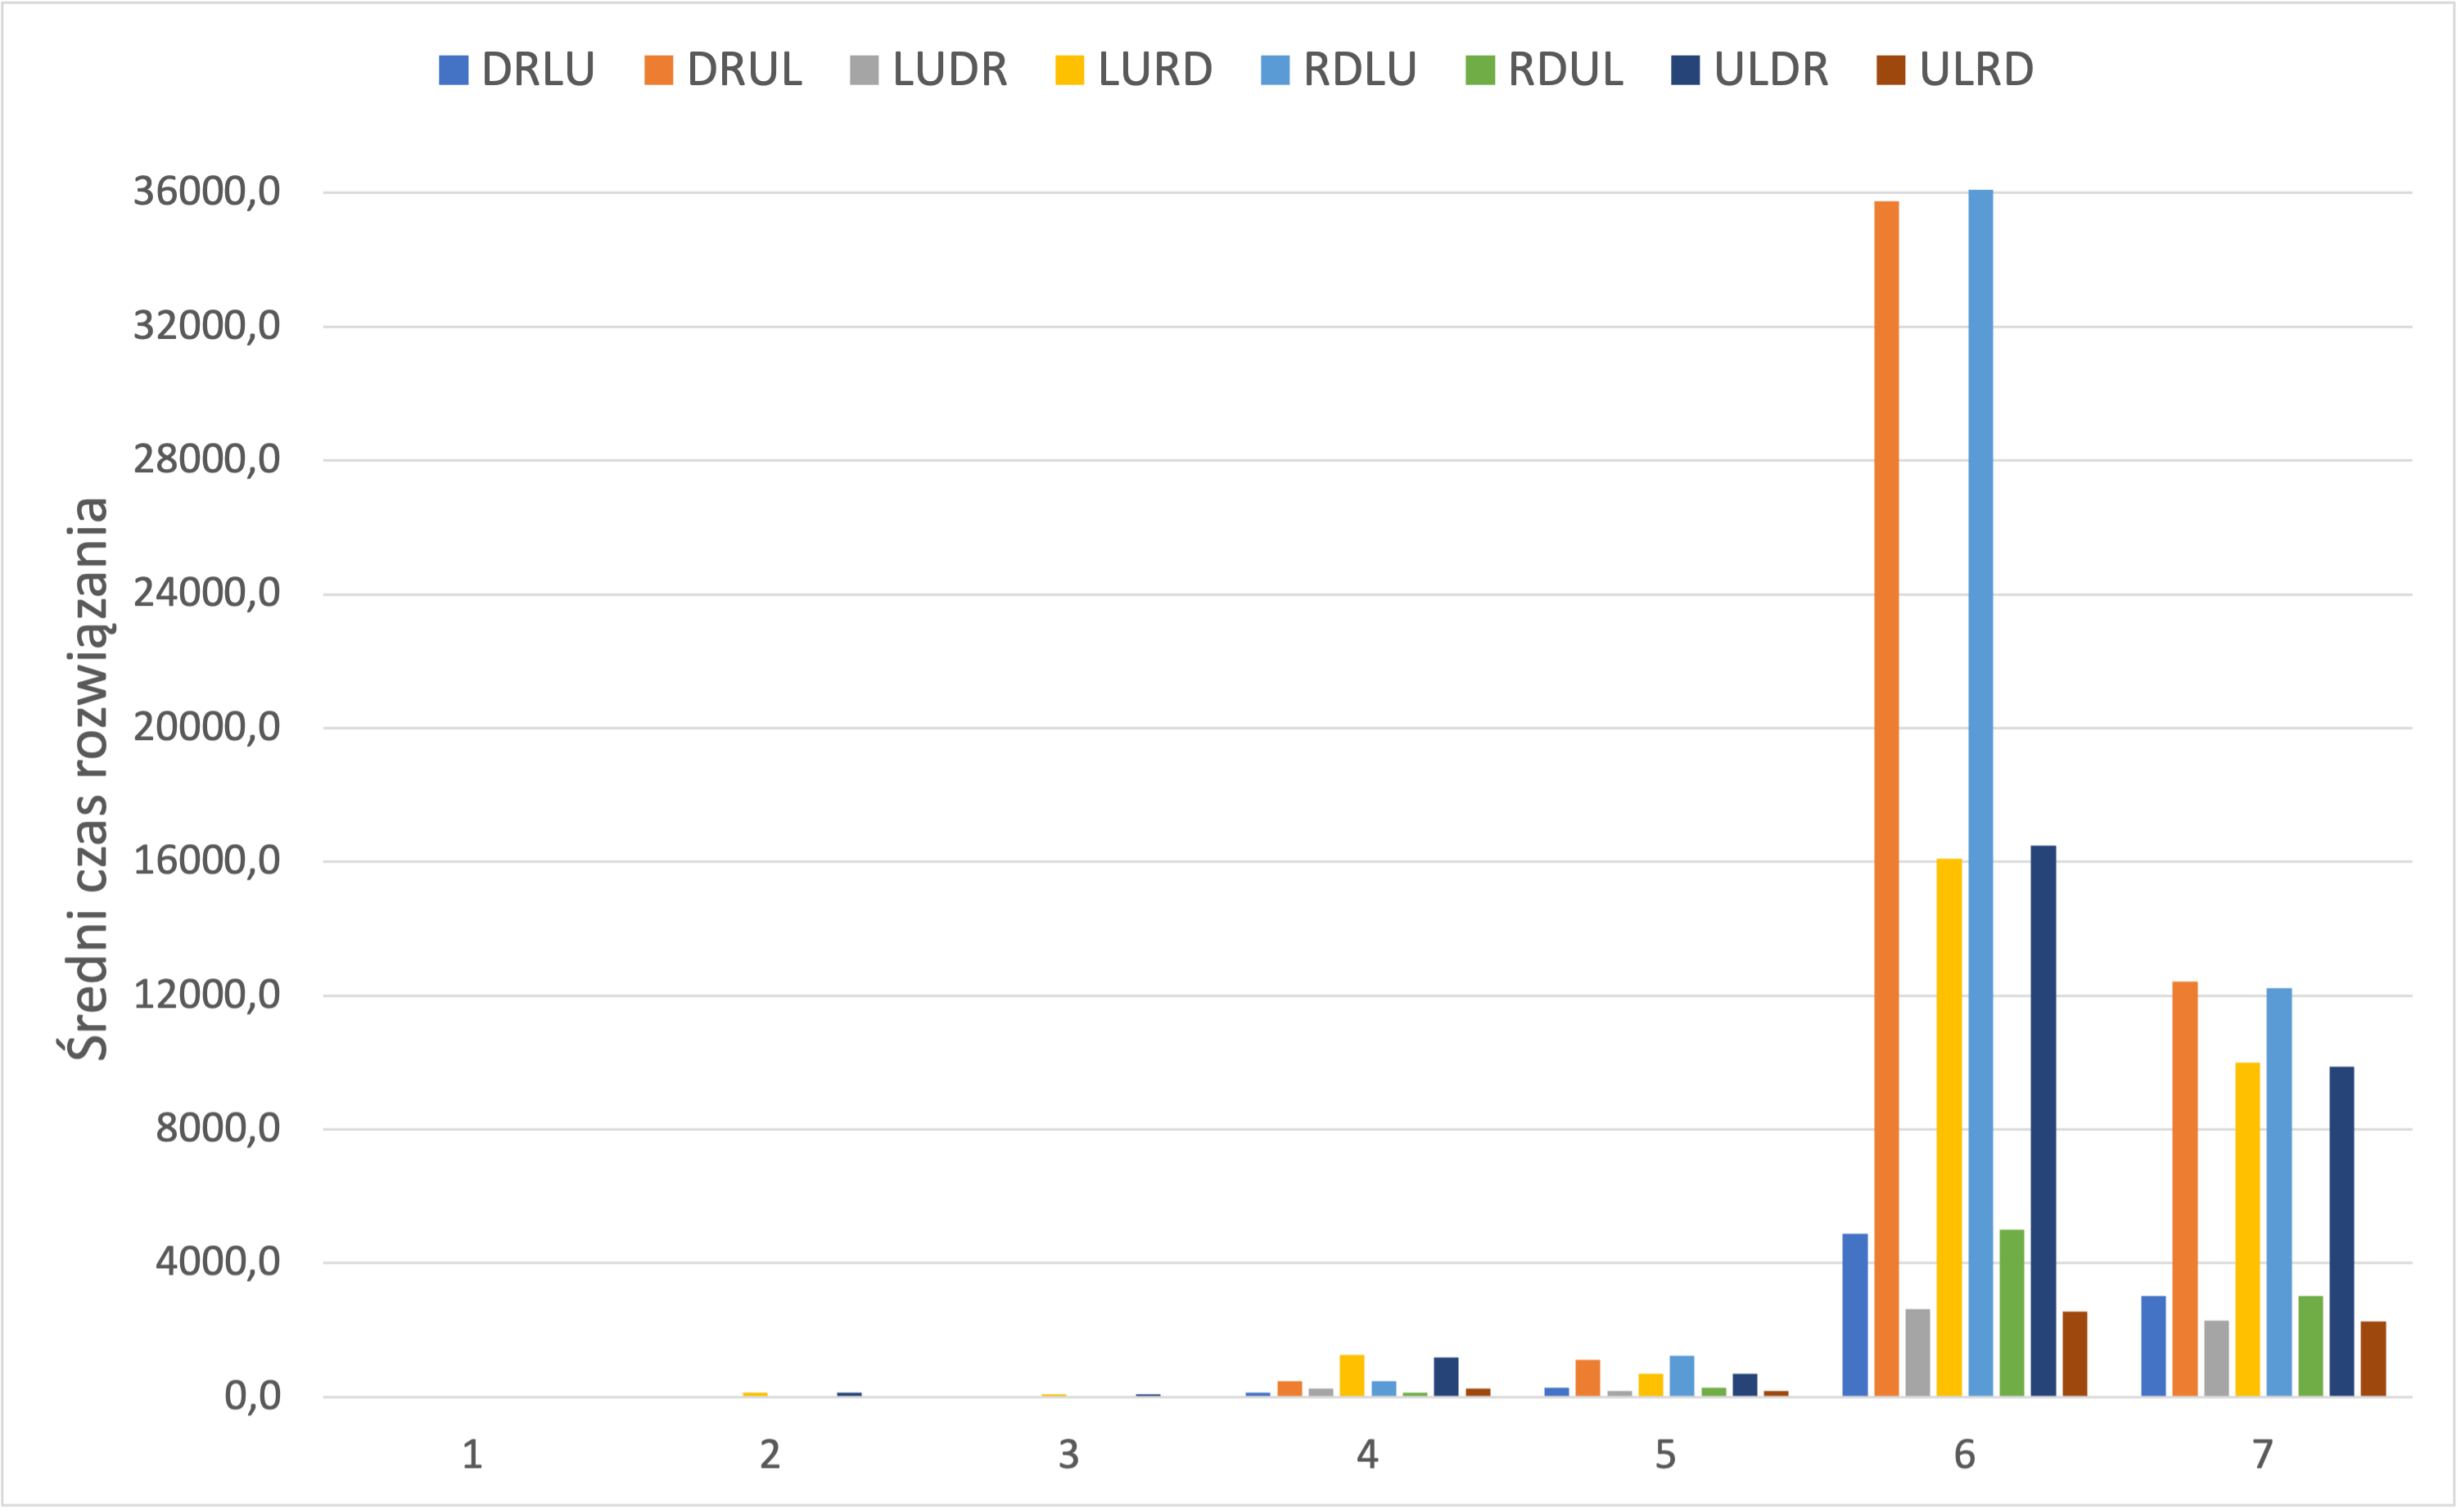
\includegraphics[width=11cm]{DFS/DFS_czas}
	\centering
	\captionsetup{name=Wykres}
	\caption{Średni czas rozwiązania dla DFS.}
	
	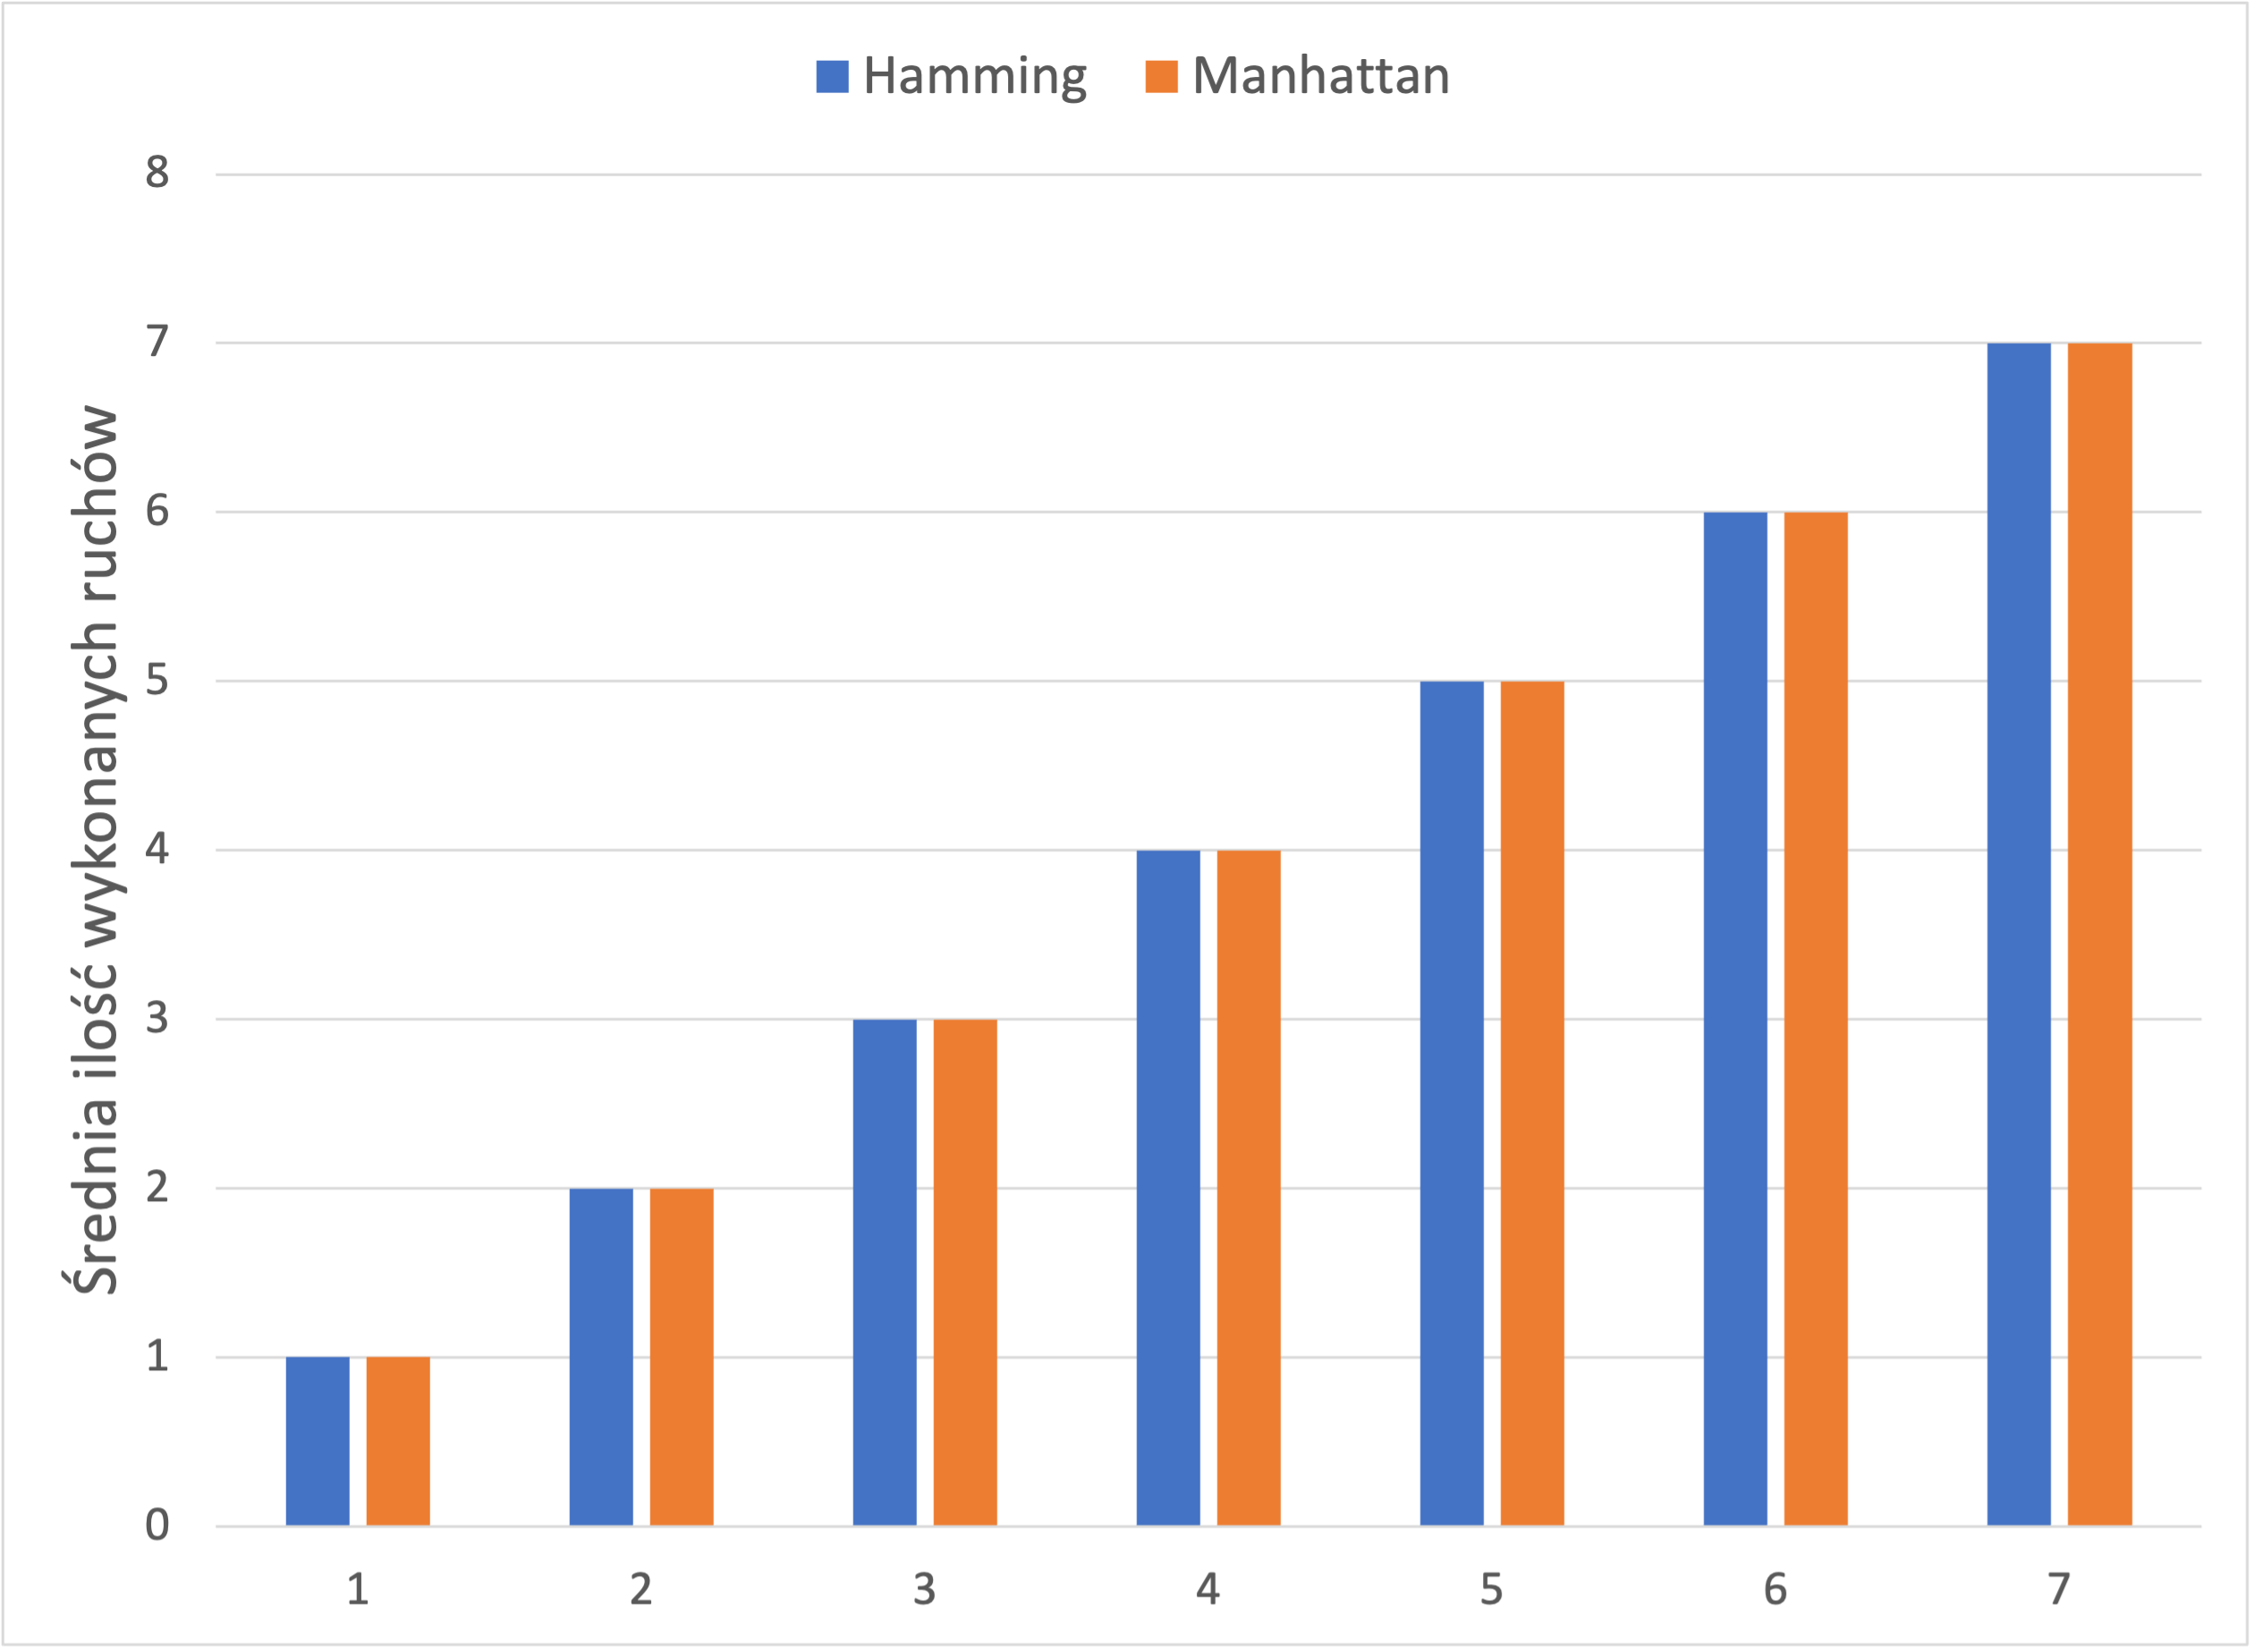
\includegraphics[width=11cm]{AStar/AStar_śr_ruchów}
	\centering
	\captionsetup{name=Wykres}
	\caption{Średnia liczba wykonanych ruchów dla A*.}
\end{figure}
\begin{figure}		
	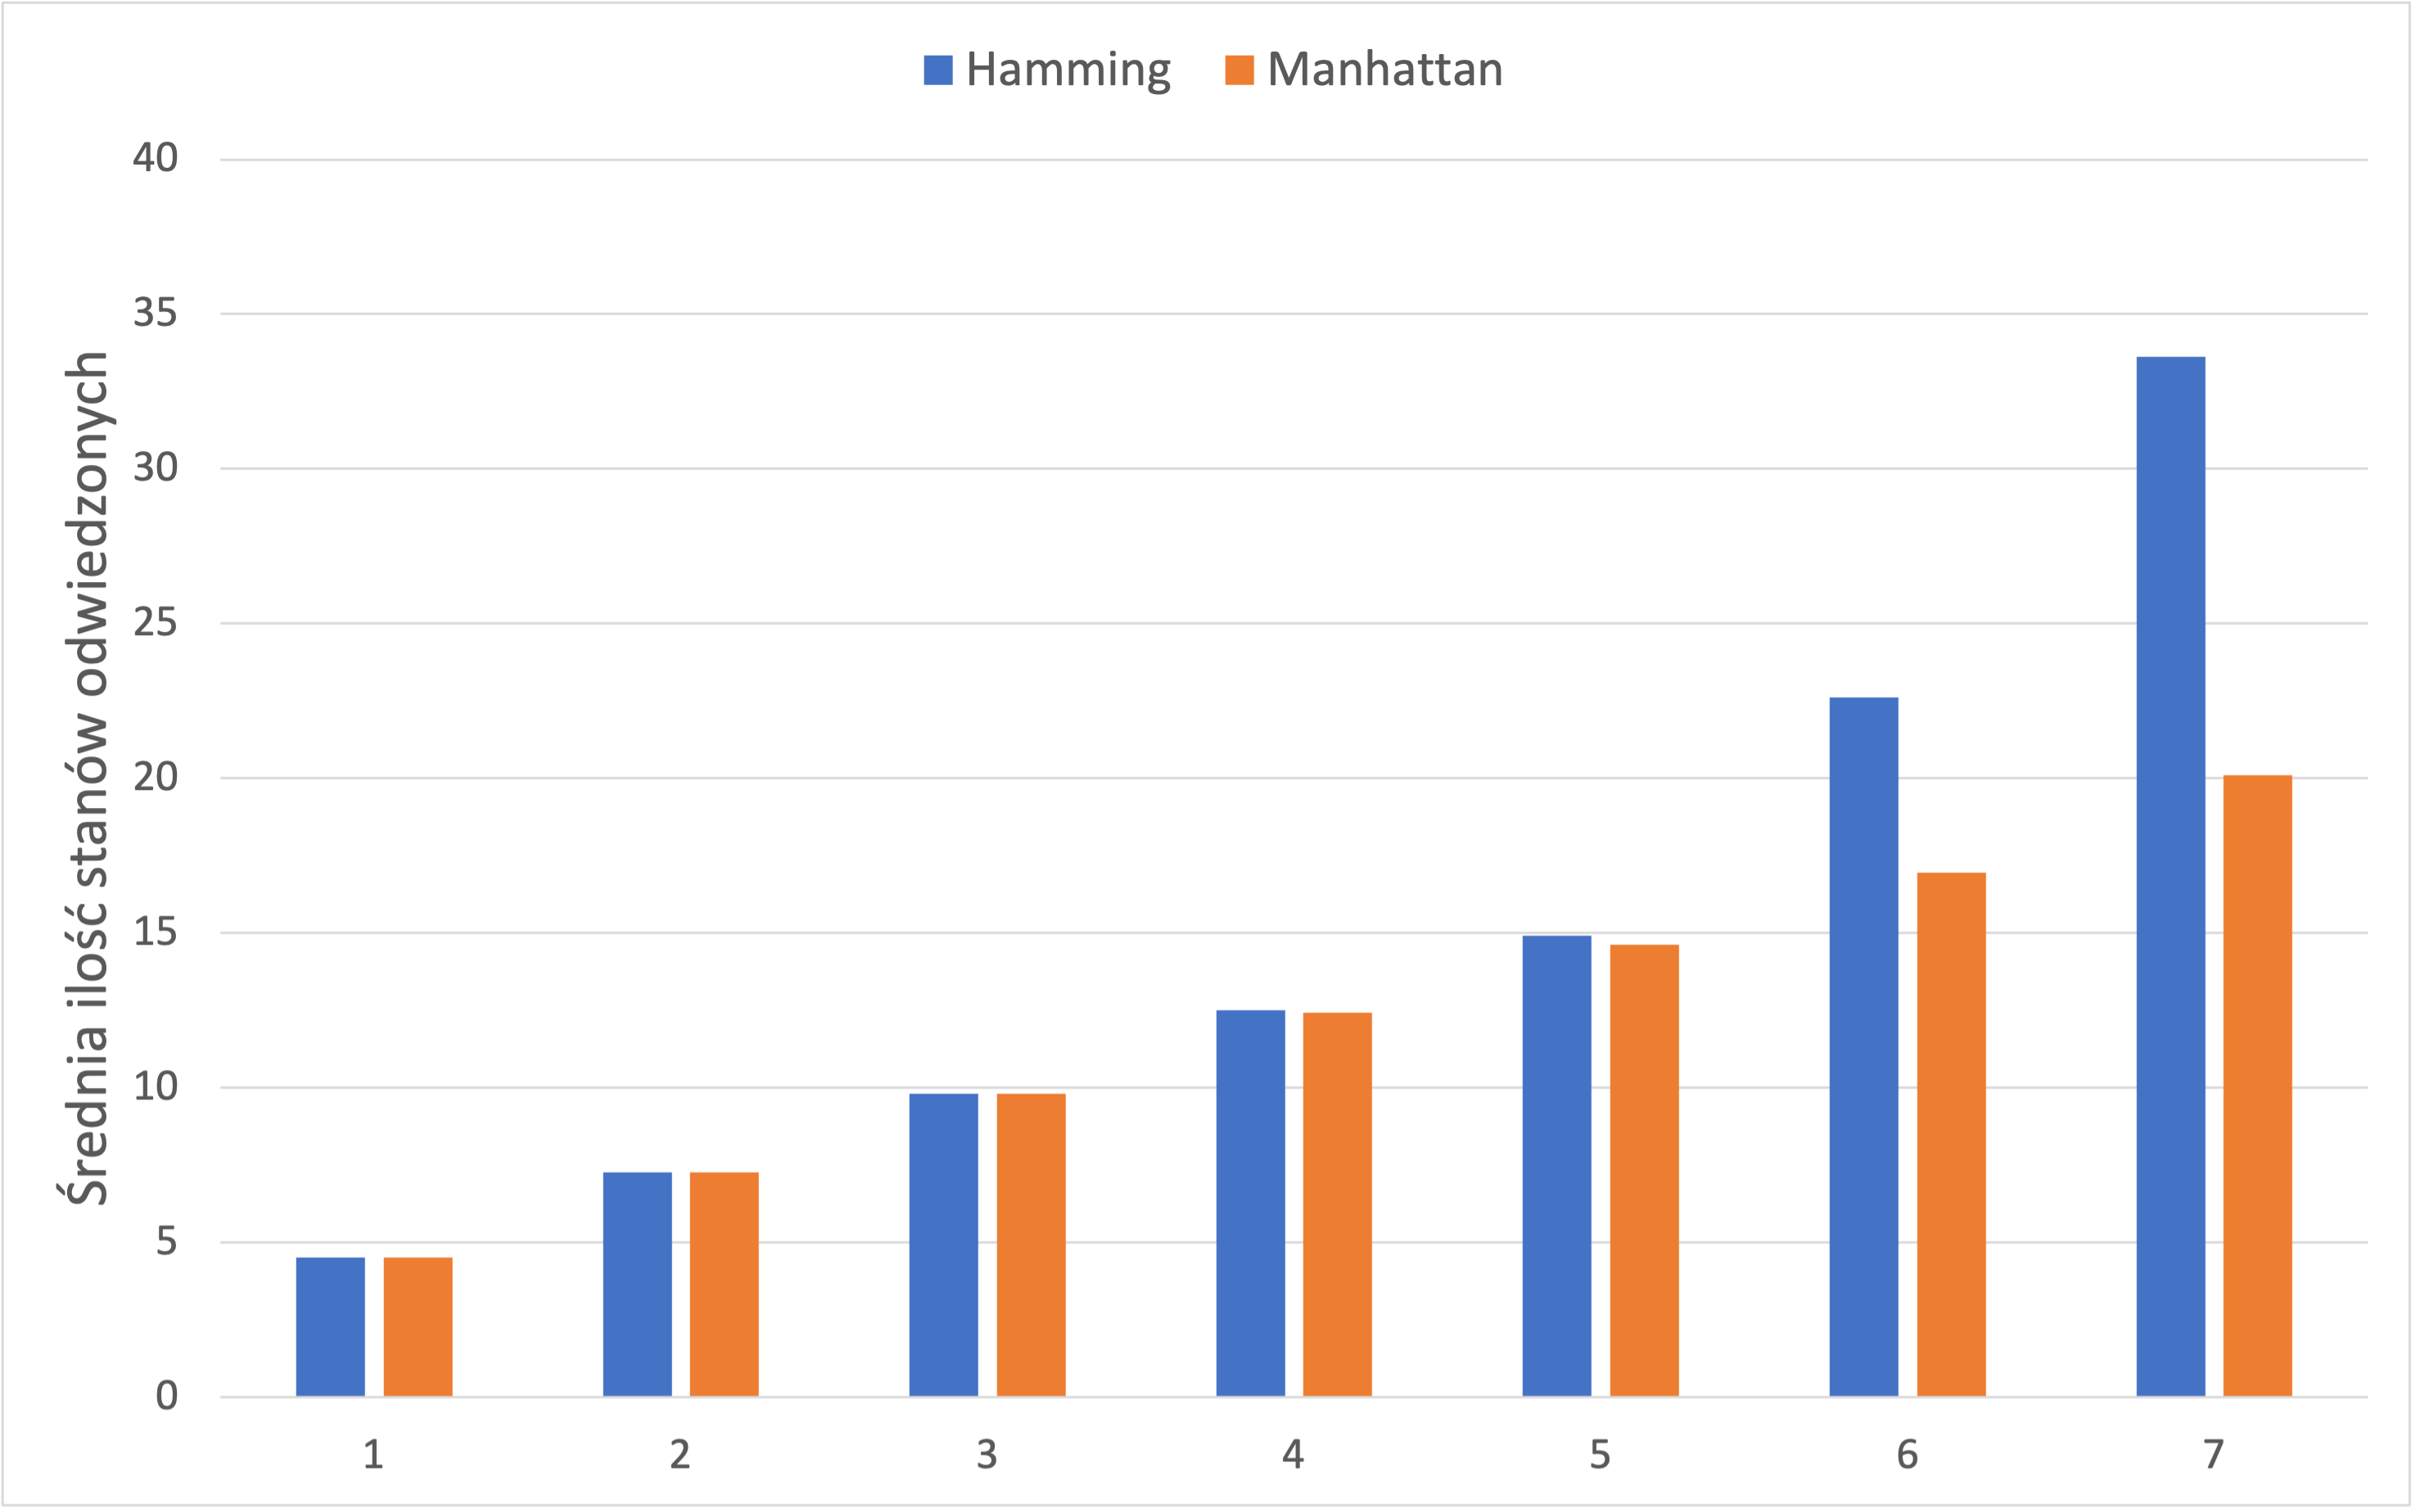
\includegraphics[width=11cm]{AStar/AStar_odwiedzone}
	\centering
	\captionsetup{name=Wykres}
	\caption{Średnia liczba odwiedzonych stanów dla A*.}
	
	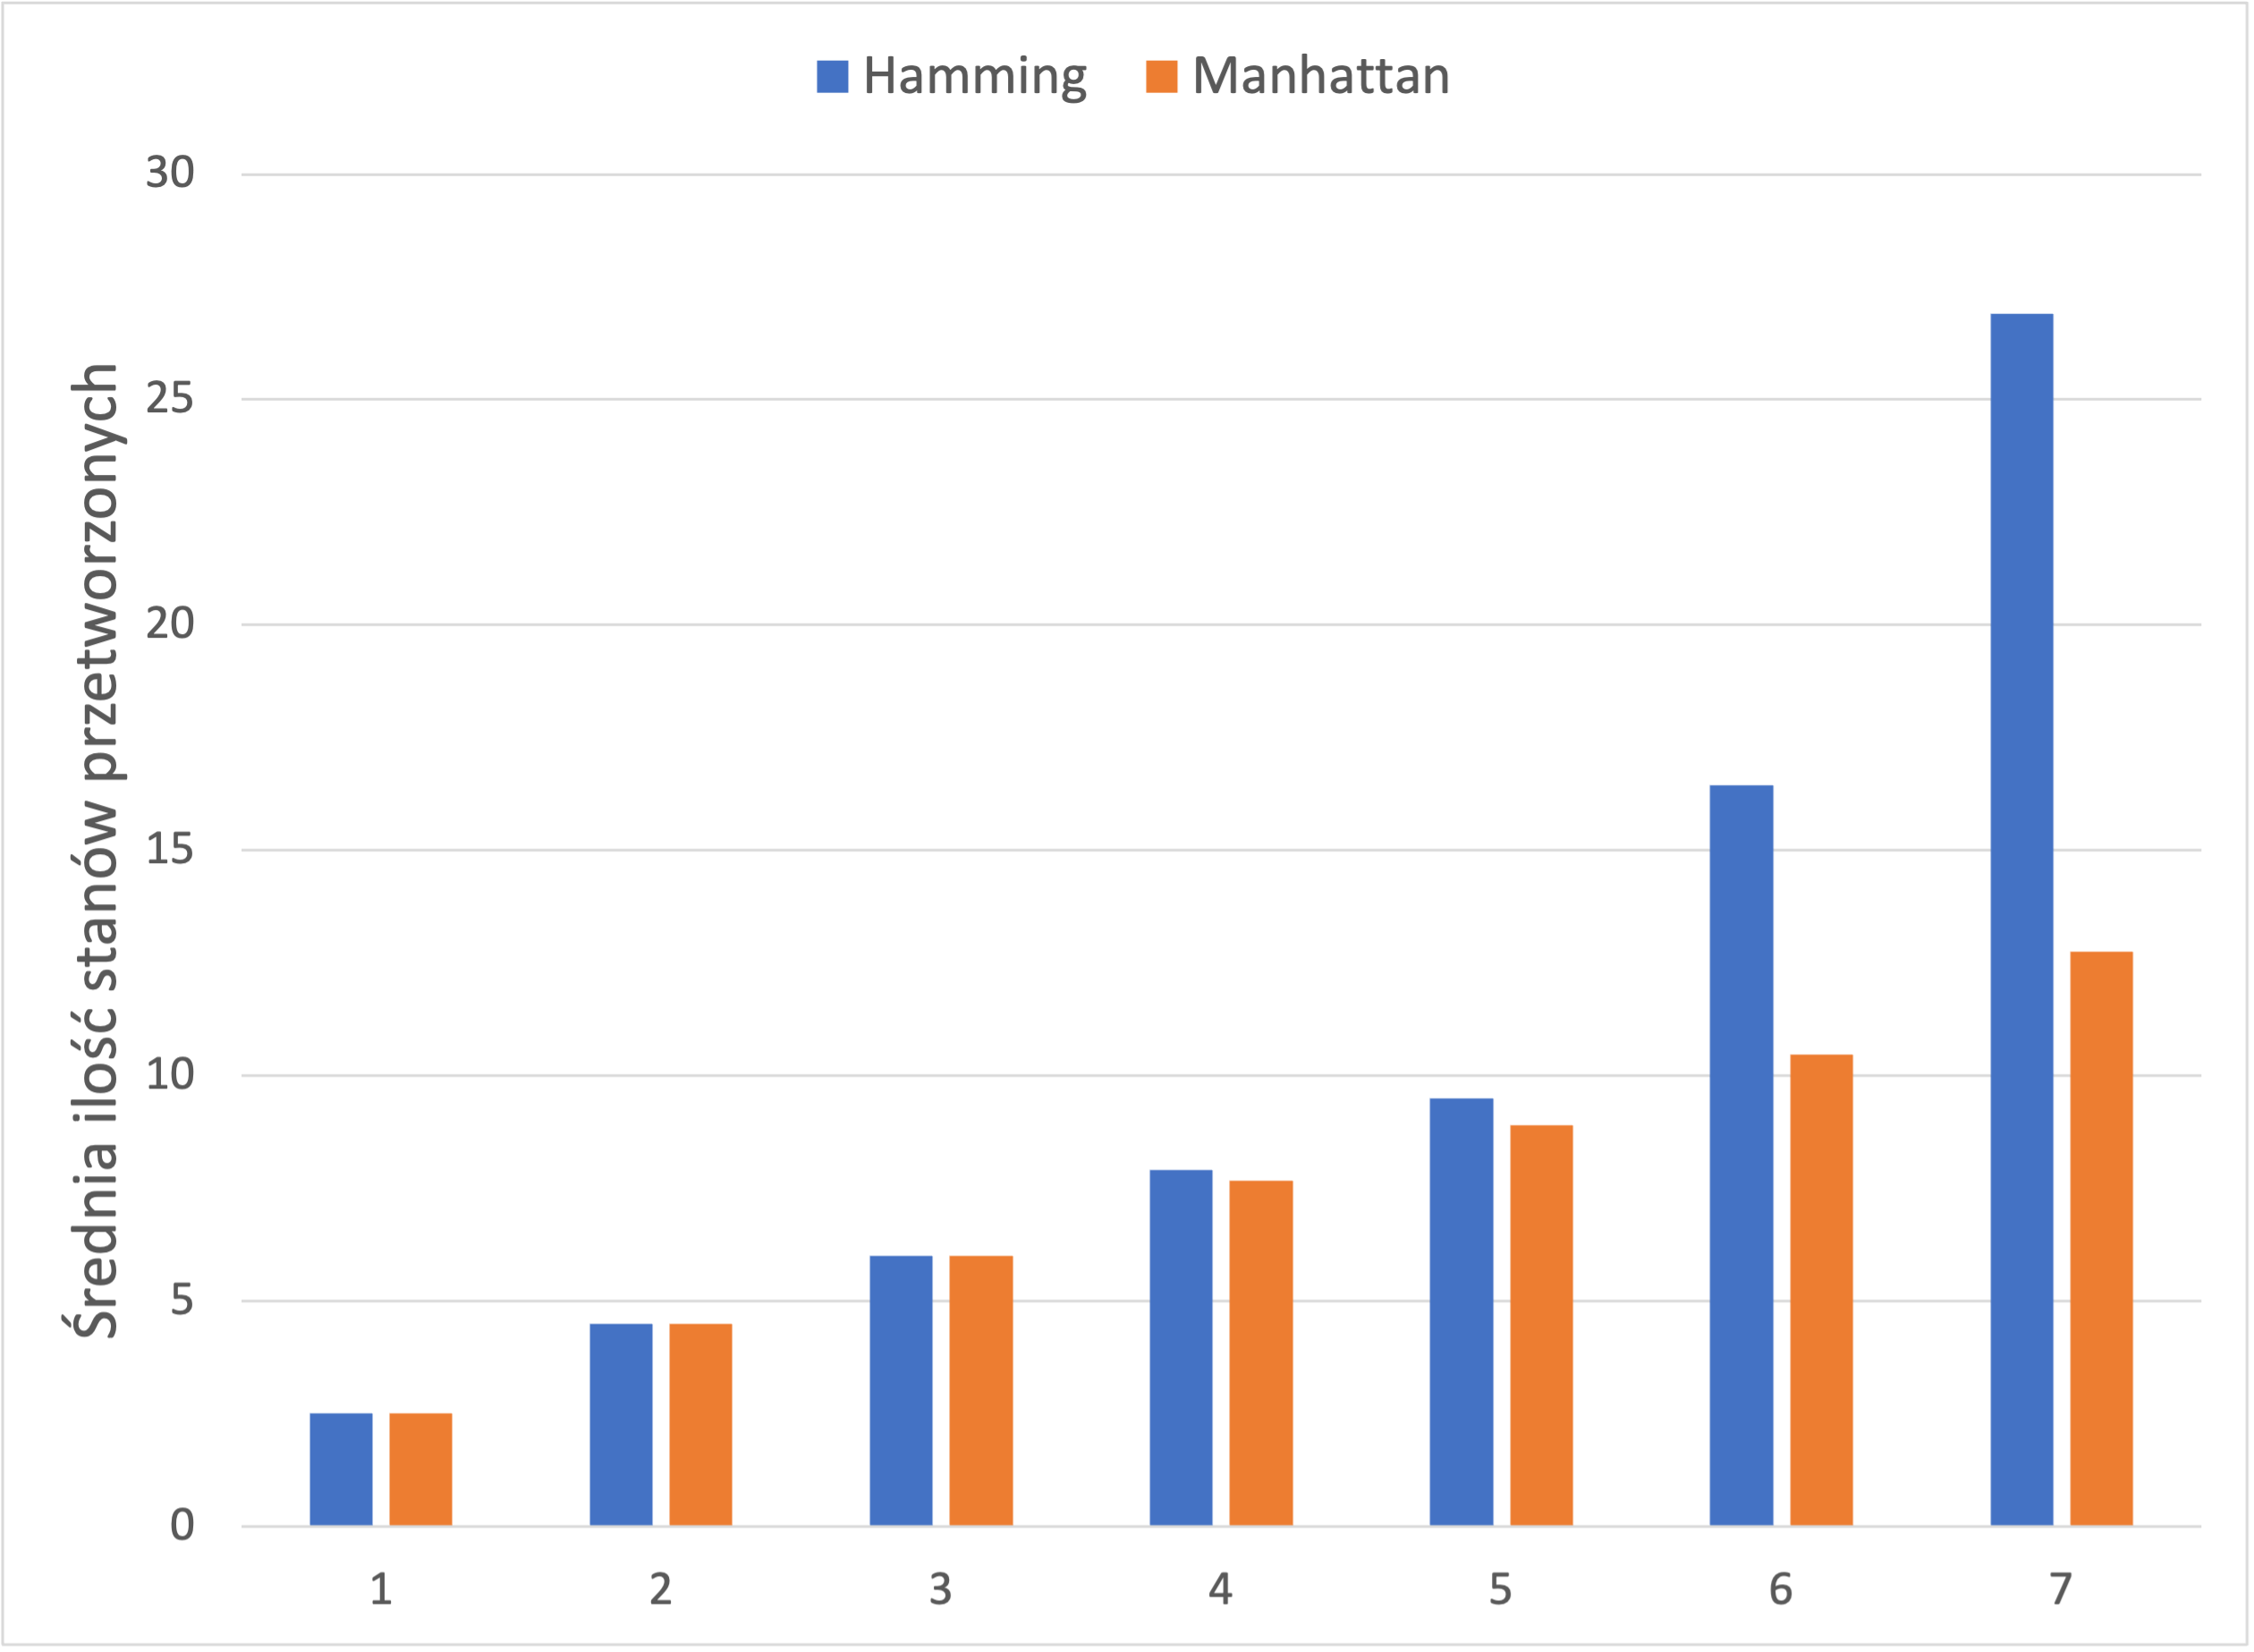
\includegraphics[width=11cm]{AStar/AStar_przetworzone}
	\centering
	\captionsetup{name=Wykres}
	\caption{Średnia liczba przetworzonych stanów dla A*.}
	
	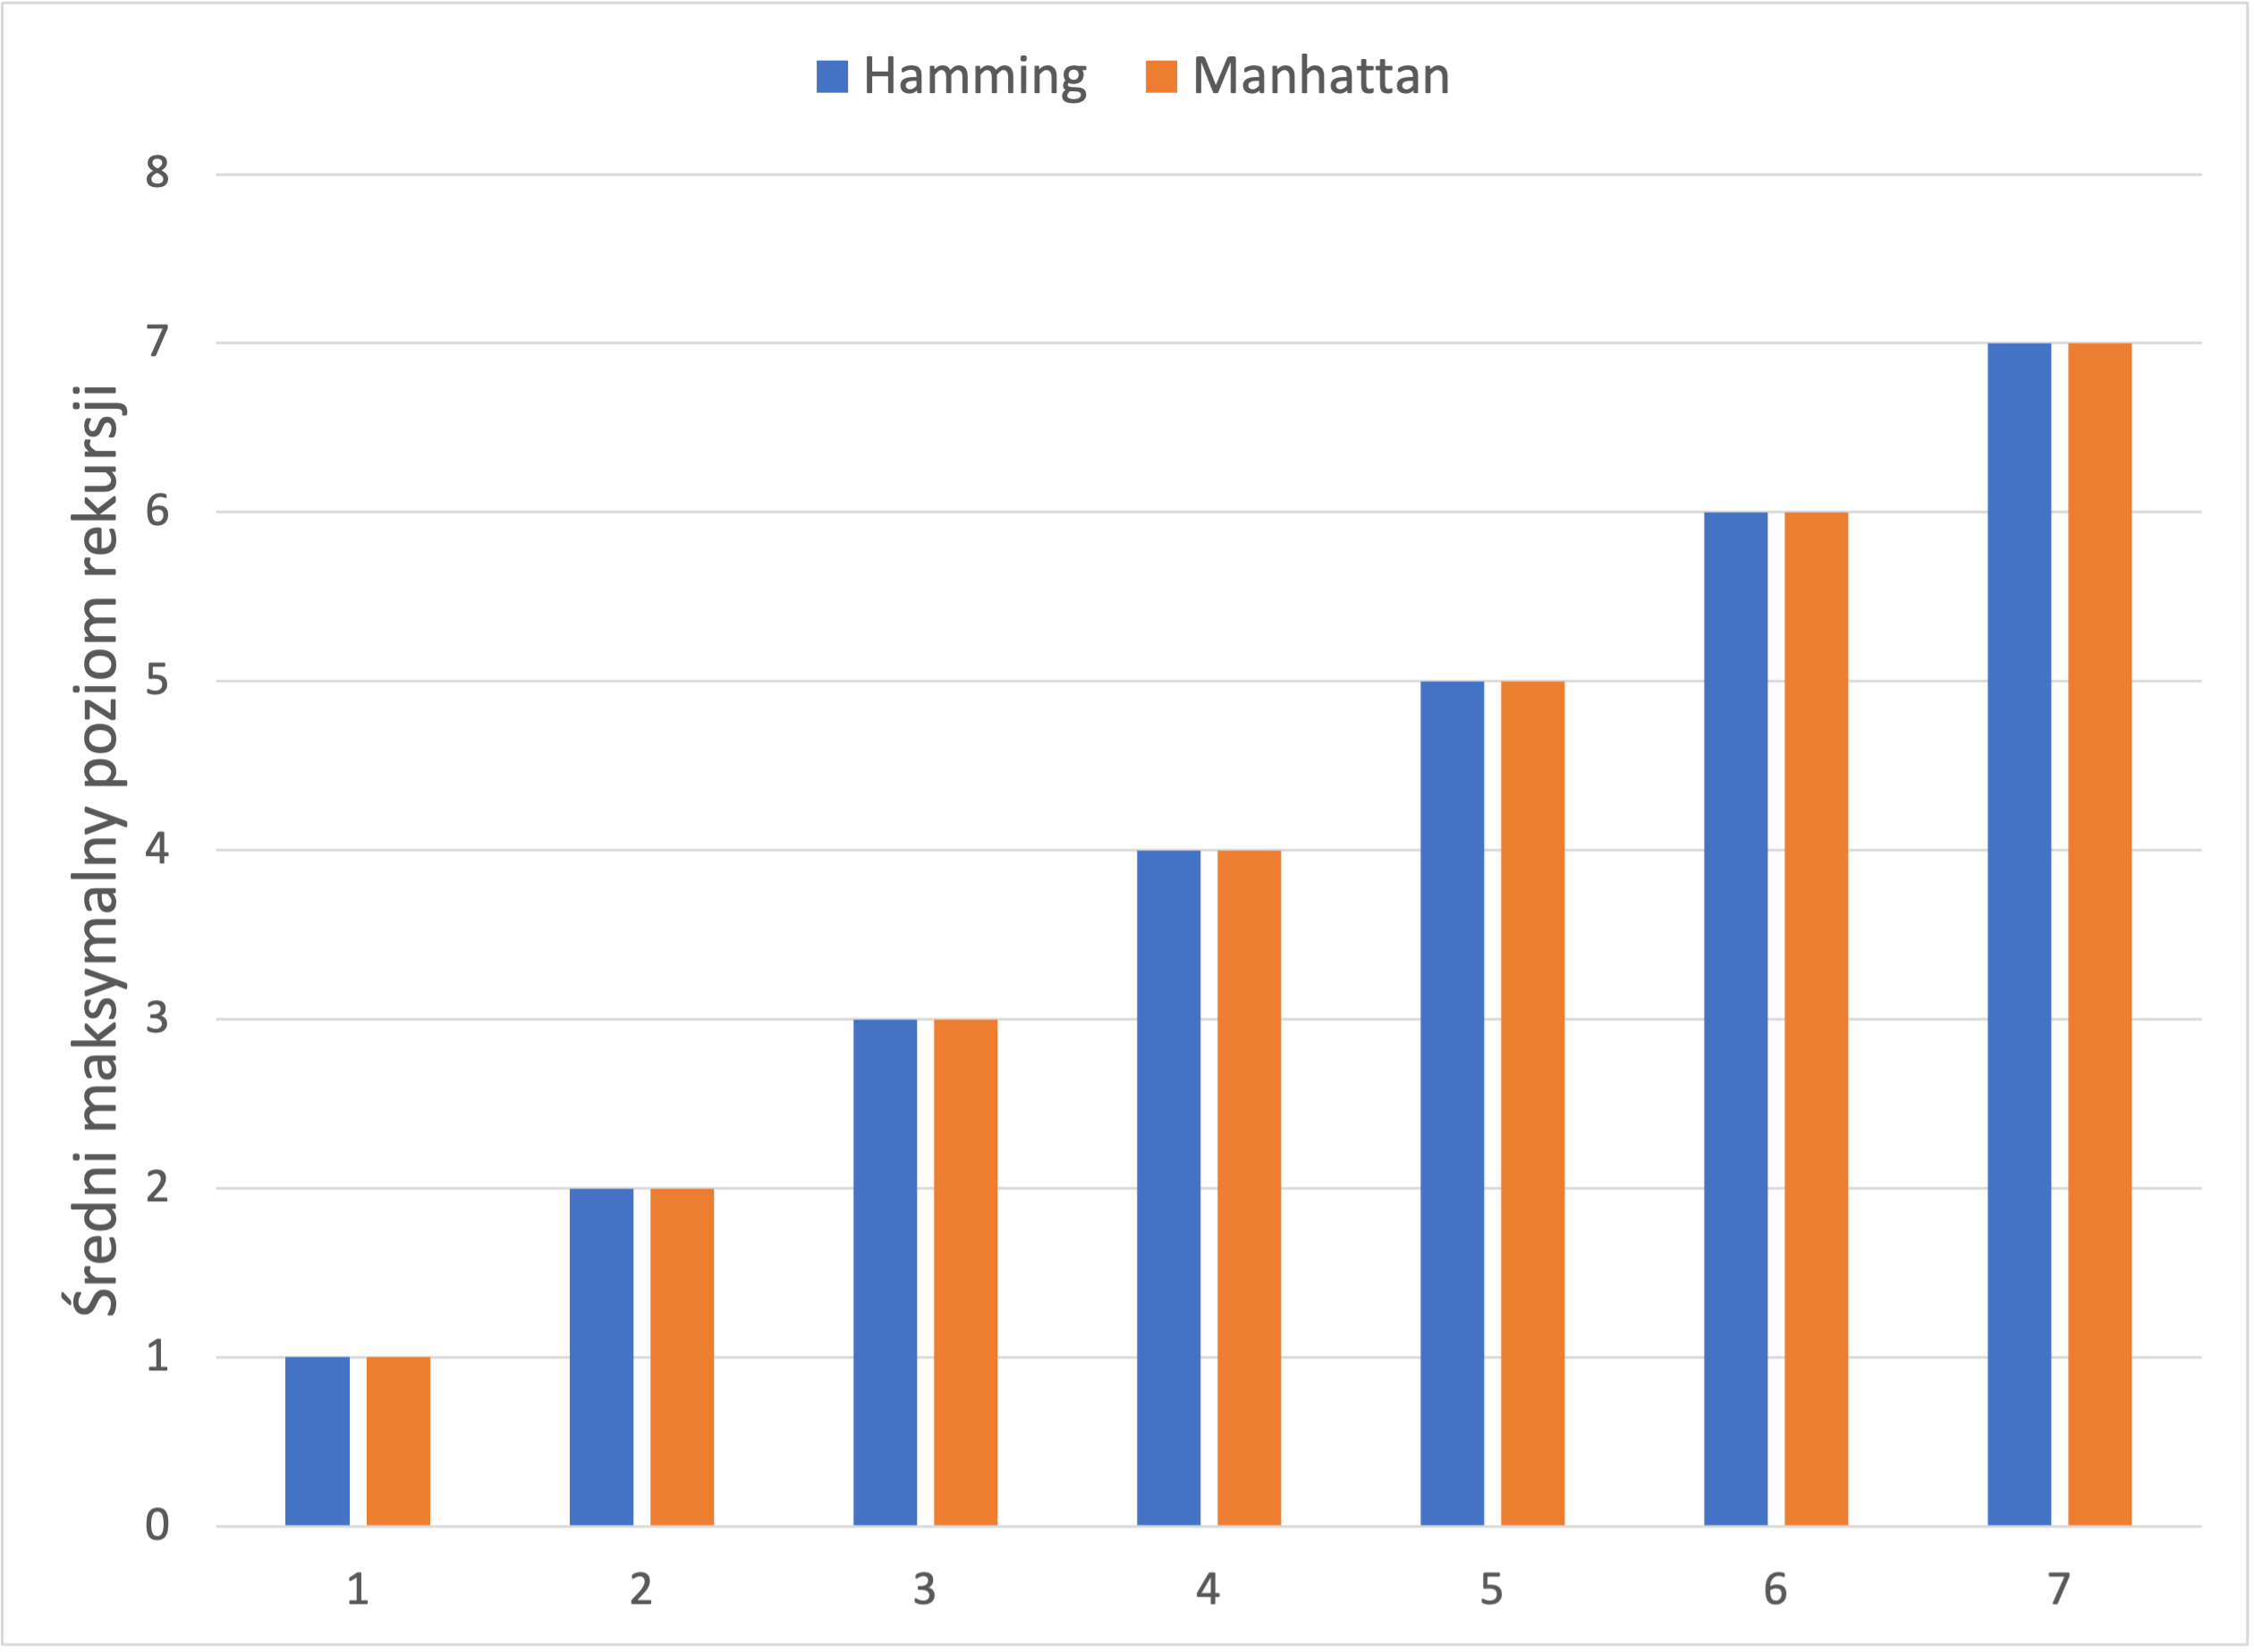
\includegraphics[width=11cm]{AStar/AStar_poziom_rekursji}
	\centering
	\captionsetup{name=Wykres}
	\caption{Średni maksymalny poziom rekursji dla A*.}
\end{figure}
\newpage
\begin{figure}		
	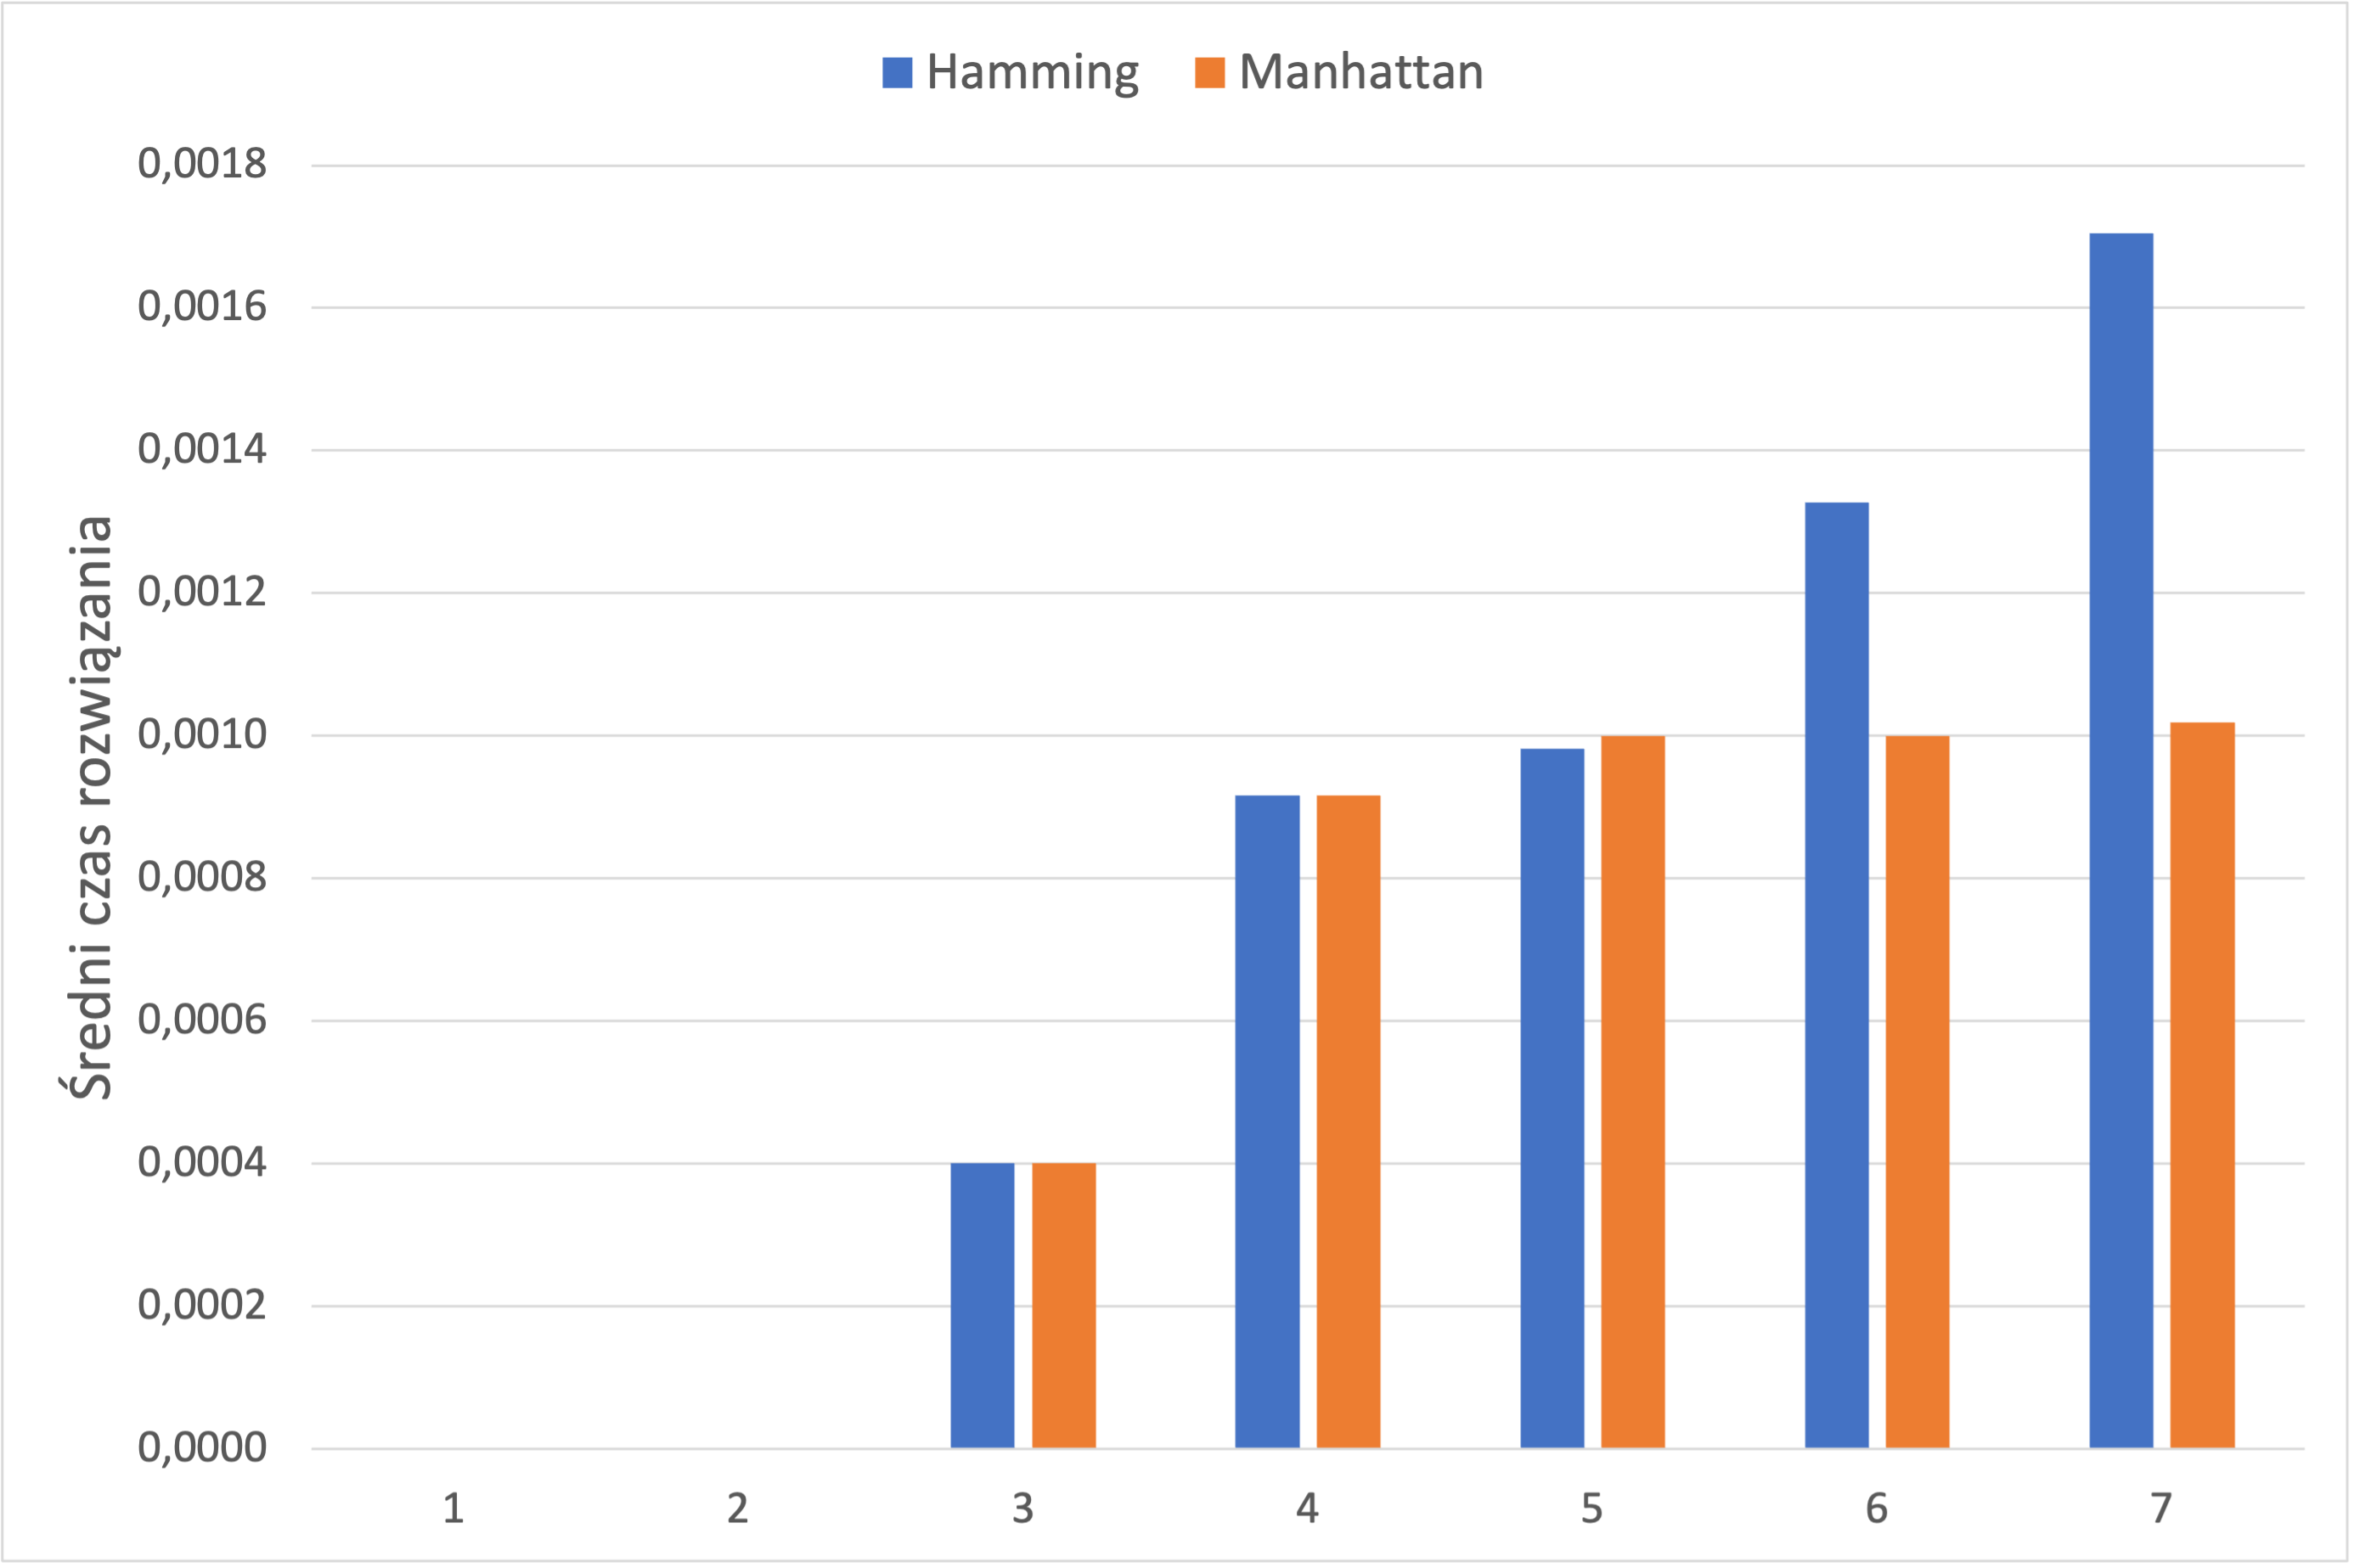
\includegraphics[width=11cm]{AStar/AStar_czas}
	\centering
	\captionsetup{name=Wykres}
	\caption{Średni czas rozwiązania dla A*.}
\end{figure}

\section{Dyskusja}
{
	\subsection{Strategia BFS}
	BFS szuka rozwiązania optymalnego, o minimalnym koszcie. \\
	Wynika to z góry ustalonego porządku, który nie pozwoli przetwarzać stanów o koszcie wyższym przed 
	przeanalizowaniem wszystkich stanów o koszcie niższym. W strategii BFS 	nigdy nie przekroczymy głębokości przy 
	przeszukiwaniu rozwiązania. BFS stosunkowo szybko znajduje rozwiązanie,
	nie biorąc pod uwagi odległości równej 7, gdzie algorytm ten potrafi znaleźć rozwiązanie znacznie wolniej od
	algorytmu A*.
	\subsection{Strategia DFS}
	Porównując DFS do pozostałych algorytmów wypada on najgorzej. \\
	Rozwiązania były optymalne dla odległości od 1 do 3, lecz dalsze trwały znacznie dłużej. Jeśli algorytm ten nie 
	potrafi znaleźć rozwiązania przy pierwszych kilku iteracjach, to odbiega on znacząco od prawidłowego rozwiązania, 
	praktycznie prawie dochodząc do maksymalnej dopuszczalnej głębokości rekursji, przetwarzając to kolejne stany w 
	okolicach tej głębokości, aż do znalezienia rozwiązania.
	\newpage
	\subsection{Strategia A*}
	Algorytm A* jest najbardziej optymalny pod względem odwiedzonych\\
	i przetworzonych stanów. Wynika to z faktu, że w 
	A* kolejność stanów do przetwarzania jest ustalana na podstawie heurystyki, a nie na z góry ustalonego porządku,
	tak jak ma to miejsce w strategiach BFS i DFS. Różnice w heurystykach nie różniły się od siebie znacząco w 
	odległościach od 1 do 5, natomiast widać różnicę na odległościach 6 i 7, gdzie metoda Hamminga odbiega od wyników 
	metody Manhattan przy odwiedzonych i przetworzonych stanach, jak i również w czasie rozwiązania.
}

\section{Wnioski}
\begin{itemize}
	\item Wydajność strategii BFS znacząco spada wraz ze wzrostem odległości od układu wzorcowego.
	\item Algorytm BFS gwarantuje znalezienie najkrótszego rozwiązania.
	\item DFS jest strategią najmniej optymalną i już na początku potrafi odbiec bardzo daleko od rozwiązania, co 
	powoduje przetwarzanie dużej ilości stanów.
	\item Algorytm DFS jest najwolniejszym ze wszystkich.
	\item W strategii A* różnice pomiędzy heurystykami zazwyczaj są nieznaczne, lecz mogą się od siebie różnić w 
	zależności od odległości badanego układu.
\end{itemize}

\begin{thebibliography}{0}
  \bibitem{l2short} \url{https://www.overleaf.com/learn/latex/Tutorials}
  \bibitem{l2short} \url{https://www.geeksforgeeks.org/breadth-first-search-or-bfs-for-a-graph/}
  \bibitem{l2short} \url{https://www.geeksforgeeks.org/depth-first-search-or-dfs-for-a-graph/}
  \bibitem{l2short} \url{https://www.geeksforgeeks.org/a-search-algorithm/}
  \bibitem{l2short} \url{https://en.wikipedia.org/wiki/Hamming_distance}
  \bibitem{l2short} \url{https://inventwithpython.com/recursion/chapter12.html}
  \bibitem{l2short} \url{https://ftims.edu.p.lodz.pl/mod/page/view.php?id=47860}
  \bibitem{l2short} \url{https://ftims.edu.p.lodz.pl/course/view.php?id=16#section-1}
\end{thebibliography}

\end{document}
